\chapter{Mathematics}
% Reason why we need a math-chapter in a book like this:
How much mathematics is needed to understand zero knowledge proofs? The answer, of course, depends on many things like the level of detail the reader want to understand them. For example it is possible to describe those proofs not using mathematics at all. However to read a foundational paper like [GROTH16], enough mathematics is needed to at least understand the basic concepts. 

Otherwise any student who is interested in learning the concepts, but who
has never seen or played with, say, a finite field, or an elliptic curve, may quickly become overwhelmed. This is not so much due to the complexity of the mathematics needs but perhaps more because of the vast amount of technical jargon, of unknown terms, obscure symbols that quickly makes a text ubreadable, desipte the concepts being actually not that hard. As a result the reader might either loose interest, or gain some dangerous smattering that in a worst case scenario materialize in inmature code. 

In this chapter we therefore derive the mathematical concepts needed to understand the basic concepts underlying snark development and we encourage the reader who is not familiar with basic number theory and lliptic curves to take the time and read this chapter until they are able to at least solve most of the simple exercises. 

If on the other hand the reader is already skilled in elliptic curve cryptography they might skip this section and only come back for reference and comparision. Maybe the most interesing parts are XXX.

We start at a very basic level and only really requie fundamntal concepts like integer arithmetics. At the same time we'll have a focus on teaching the reader how to think mathematically and to understand that there are numbers and methatical structures out there that appear to be very different from the stuff we learned in school and yet on a deeper level they are in deed very similar.

We want to stress however, that our introduction is informal, incomplete and optimized to enable the reader to understand zero knowledge concepts as efficient as possible. Our focus and design choices are so that we give as little theory as necessary but accompanied by a wealth of numerical examples. We found this on the believe, that such an informal, example-
driven approach to learning mathematics may ease the beginner’s digestion in the initial stages. 

For instance, a beginner would be likely to find it more beneficial to first compute a simple toy snark in a pen and paper style all the way through all steps before they dig deeper and actually devop real world production ready systems. Also having already a few simple examples in you head, its likely easier to only then read the actual academic papers. 

However in order to be able to derive those toy example, some mathematical groundwork is needed. This chapter therefore will help the reader to focus on what is important, while at the same time serve as first exercises the reader is encouraged to recompute themself. Every section usually then ends with a list of additional exercises in increasing difficulty order, to help the reader memorising and applying the concepts given. 

Overall the goal of this chapter is to provide a reader who is starting with nothing more than basic high school algebra, to be able to solve basic tasks in elliptic curve cryptography without the need of a computer.


%Summary of this chapter
We start with a brief recapitulation of basic integer aithmetics like long division, the greatest common divisior and Euklids algorithm. After that we introduce modular arithmetics as \textbf{the most important} skill to compute our pen and paper examples. We then introduce polynomials, compute their analogs to integer arithmetics and introduce the important concept of Lagrange interpolation.

After this practical warm up, we have to introduce some basic algebraic terms like groups and fields, because those terms are all over the place when reading academic papers in the context of zero knowledge proof. The beginner is good adviced to memorize those terms and think about them. We define these terms in the general abstract way of mathematics, hoping that the non mathematical trained reader will gradually learn to become comfortable with this style. We then give basic examples and do basic computations with these examples to get familiar with the concepts. 

\section{Integer Arithmetics}
\label{integer_arithmetics}
To some degree, most readers with probably remember integer arithmetics from school. It is however important for the rest of the book to be able to apply those concepts to understand and execute computations in the various pen and paper examples that are the main contribution of the moon math manual. We will therefore recapitulate those concepts filling up some knowledge gaps.

In what follows we applay standard mathematical notations and use the symbol $\mathbb{Z}$ for the set of all integers, that is we write
\begin{equation}
\label{integer_symbol}
\Z := \{\ldots, -3,-2,-1,0,1,2,3,\ldots\}
\end{equation}
So whenever you see the symbol $\mathbb{Z}$, think of the set of all integers. If $a \in \Z$ is an integer, we write $|a|$ for the \textit{absolute value} of $a$, that is the the non-negative value of $a$ without regard to its sign. In addition we will use the symbol $\N$ for the set of all counting numbers, that is we write 
\begin{equation}
\label{integer_symbol}
\N := \{0,1,2,3,\ldots\}
\end{equation}
including the number $0$. So whenever you see the symbol $\mathbb{N}$, think of the set of all non negative integers. 

To make it easier to memorize new concepts and symbols, we might frequently link to definitions (See \ref{integer_symbol} for a definition of $\Z$) in the begining, but as to many links render a text unreadable, we will assume the reader will become familiar with definitions as the text proceeds at which point we will not link them anymore. 

Both sets $\N$ and $\Z$ have a notion of addition as well as multiplication dedined on them and also most of us are probably able to do many integer computations in their head, we will frequently invoke the sagemath system (\ref{sagemath_setup}) for more complicated computations. One way to invoke the integer-type in sage is:
\begin{sagecommandline}
sage: ZZ # A sage notation for the integer type
sage: NN # A sage notation for the counting number type
sage: ZZ(5) # Get an element from the Ring of integers
sage: ZZ(5) + ZZ(3)
sage: ZZ(5) * NN(3)
sage: ZZ.random_element(10**50)
sage: ZZ(27713).str(2) # Binary string representation
sage: NN(27713).str(2) # Binary string representation
sage: ZZ(27713).str(16) # Hexadecimal string representation
\end{sagecommandline}
Of particular interest for us are the so called \textit{prime numbers}, which are counting numbers $ p \in \N $ with $ p \geq 2 $, which are divisible by themself and by $ 1 $ only. Prime numbers are called \textit{odd} if they are not the number $ 2 $. We write $ \Prim $ for the set of all prime numbers and $ \Prim _{\geq 3} $ for the set of all odd prime numbers.
$\Prim$ is infinite and can be ordered according to size, so that we can writem them as
\begin{equation}
\label{eq: primenumber_sequence}
2, 3, 5, 7, 11, 13, 17, 19, 23, 29, 31, 37, 41, 43, 47, 53, 59, 61, 67, \ldots
\end{equation}
which is sequence $ A000040 $ in OEIS. In particular, we can talk about small and large prime numbers.

As the \textit{fundamental theorem of arithmetics} tells us, prime numbers are in a certain sense the basic building blocks from which all other natural numbers are composed. To see that, let $ n \in \N_{\geq 2} $ be any natural number. Then there are always prime numbers $ p_1, p_2, \ldots, p_k \in \Prim $, such that
\begin{equation}
n = p_1 \cdot p_2 \cdot \ldots \cdot p_k \;.
\end{equation}
This representation is unique, except for permutations in the factors and is called the \textbf{prime factorization} of $n$.
\begin{example}[Prime Factorization] To see what we mean by integer factorization, lets look at the number $19214758032624000$. To get its prime factors, we can sucessively divide it by all prime numbers in ascending order starting with $2$. We get
\begin{equation*}
19214758032624000 = 2\cdot 2\cdot 2\cdot 2\cdot 2\cdot 2\cdot 2 \cdot 3\cdot 3\cdot 3\cdot 5\cdot 5\cdot 5\cdot 7 \cdot 11 \cdot 17\cdot 17 \cdot 23 \cdot 43\cdot 43 \cdot 47
\end{equation*}
We can double check our findings invoking sage, which provides an algorith to factor counting numbers:
\begin{sagecommandline}
sage: n = ZZ(19214758032624000)
sage: factor(n)
\end{sagecommandline}
\end{example}
Having done the computation from the previous example, reveals an important observation: Computing the factorization was computationally expensive, while on the other hand, giving a string of prime numbers, computing their product is fast. 

From this an important question arises: How fast we can compute the prime factorization of a natural number? This is the famous \textit{factorization problem} and as far as we know, there is no method on a classical Turing machine that is able to compute this representation in polynomial time. The fastest algorithms known today run sub-exponentially, with $\mathcal{O}((1+ \epsilon)^n)$ and some $ \epsilon> 0 $.

It follows that integer factorization $\Leftrightarrow$ prime number multiplication is an example of, what is called a one-way.function. Something that is easy to compute in one direction, but hard to compute in the other direction. Existence of one way functions like this are basic crytographic assumptions, that the security of many crypto systems is based on.

It should be pointed out however hat the American mathematician Peter Williston Shor developed an algorithm in 1994 which can calculate the prime factor representation of a natural number in polynomial time on a quantum computer. The consequence of this is, of course, that cryosystems, which are based on the time complexity of the prime factor problem, are unsafe as soon as practically usable quantum computers are available.
\begin{exercise}
Compute the factorization of $6469693230$ and double check your results using sage.
\end{exercise}

\paragraph{Euklidean Division}
\label{Euklidean_division}
In general there is no division defined in the usual sense for integers, as for example $7$ divided by $3$ will not be an integer again. However it is possible to devide any two integers with a remainder. So for example $7$ divided by $3$ is equal to $2$ with a remainder of $1$, since $7 = 2\cdot 3 + 1$. 

Doing integer division like this is probably something many of us remember from school. It is 
usually called \textit{Euclidean division}, or division with remainder and it is an important technique, that every reader must become familiar with to understand many concepts in this book. The precise definition is as follows:

Let $ a \in \Z $ and $ b \in \Z $ be two integers. Then there is always another integer $ m \in \Z $ and a counting number $ r \in \N $, with $ 0 \leq r <|b| $ such that
\begin{equation}
\label{eq_euklidean_division}
a = m \cdot b + r
\end{equation}
This decomposition of $a$ given $b$ is called \textit{Euklidean division}, where $ a $ is called the \textit{divident}, $ b $ is called the \textit{divisor}, $m$ is called the \textit{quotient} and $r$ is called the \textit{remainder}. 
\begin{notation}
\label{eq_euklidean_division_notation}
Suppose that the numbers $ a, b, m $ and $ r $ satisfy equation (\ref{eq_euklidean_division}). Then we often write 
\begin{equation}
\label{def_integer_division_and_modulus}
\begin{array}{lcr}
\Zdiv{a}{b}: = m, & & \Zmod{a}{b}: = r 
\end{array}
\end{equation}
to describe the quotient and the remainder of the Euklidean division. We also say, that an integer $ a $ is divisible by another integer $ b $ if $ \Zmod{a}{b} = 0 $ holds. In this case we also write $ a | b $.
\end{notation}
So in a Nutshell Euclidean division is a process of dividing one integer by another, in a way that produces a quotient and a non negative remainder the latter of which is smaller than the absolute value of the divisor. It can be shown, that both the quotient and the remainder always exist and are unique, as long as the divident is different from $0$.

A special situation occures, is the remainder is zero, because in this special case the divident \textit{is} divisible by the divisor. Our notation $a|b$ refelcts that. 


\begin{example} Applying Euklidean division and our previously defined notation \ref{def_integer_division_and_modulus} to the divisor $-17$ and the divident $4$, we get 
\begin{equation*}
\begin{array}{lcr}
\Zdiv{-17}{4} = - 5, & & \Zmod{-17}{4} = 3
\end{array}
\end{equation*}
because $ -17 = -5 \cdot 4 + 3 $  is the Euklidean division of $-17$ and $4$ (Since the remainder is by definition a non-negative number). In this case $4$ does not divide $-17$ as the reminder is not zero. Writing $-17 | 4$ therefore has no meaning. On the other hand we can write $12 | 4$, since $4$ divides $12$, as $ \Zmod{12}{4} = 0 $. We can invoke sagemath to do the computation for us. We get
\begin{sagecommandline}
sage: ZZ(-17) // ZZ(4) # Integer quotient 
sage: ZZ(-17) % ZZ(4) # remainder 
sage: ZZ(4).divides(ZZ(-17)) # self divides other
sage: ZZ(4).divides(ZZ(12))
\end{sagecommandline}
\end{example}
Methods to compute Euklidean division for integers are called \textit{integer division algorithms}. Probably the best known algorithm is the so called \textit{long division}, that most of us might have learned in school. It should be noted however that there are faster methods like \textit{Newton–Raphson division}.

As long division is the standard method used for pen-\&-paper division of multi-digit numbers expressed in decimal notation, the reader should become familiar with it as we use it all over this book when we do simple pen-and-paper computations. However instead of defining the algorithm formally, we rather give some examples, that hopelly will make the process clear

\begin{example}[Integer Long Division] To give an example of integer long division algorithm, lets divide the integer $a=143785$ by the number $b=17$. Our goal is therfore to find solutions to equation \ref{eq_euklidean_division}, that is we need to find the quotient $m\in\Z$ and the reminder $r \in \N$ such that $143785 = m\cdot 17 + r$. Using a notation that is mostly used in Commonwealth countries, we compute
\begin{equation}
\intlongdivision{143785}{17}
\end{equation}
We therefore get $m=8457$ as well as $r=16$ and indeed we have $143785 = 8457\cdot 17 + 16$, which we can double check invoking sage:
\begin{sagecommandline}
sage: ZZ(143785).quo_rem(ZZ(17)) # Euclidean Division
sage: ZZ(143785) == ZZ(8457)*ZZ(17) + ZZ(16) # check
\end{sagecommandline}
In a nutshell, the algorithm loops through the digits of the divident from the left to right, subtracting the largest possible multiple of the divisor (at the digit level) at each stage; the multiples then become the digits of the quotient, and the remainder is the first digit of the divident.
\end{example}
\begin{exercise}[Integer Long Division]
Find an $m\in\Z$ as well as an $r\in\N$ such that $a= m\cdot b +r$ (See equation \ref{eq_euklidean_division}) holds for the folling pairs $(a,b) = (27,5)$, $(a,b)=(27,-5)$, $(a,b)=(127,0)$, $(a,b)= (-1687, 11)$. In which cases are your solutions unique?
\end{exercise}
\begin{exercise}[Long Division Algorithm]
Write an algorithm in pseudocode that computes integer long division, handling all edge cases properly.
% https://en.wikipedia.org/wiki/Division_algorithm
\end{exercise}

\paragraph{The Extended Euklidean Algorithm}
One of the most critical parts in this book is modular arithmetics XXX and its application in the computations in so called finite fields, as we explain in XXX. In modular arithmetics it is sometimes possible to define actual division and multiplicative inverses of numbers, that is very different from inverses as we know them from other systems like factional numbers. 

However, to actually compute those inverses we have to get familar with the so-called \textit{extended Euclidean algorithm}. To recapitulate jargon first, the \textit{greatest common divisor} (GCD) of two nonzero integers $a$ and $b$ is the greatest non-zero counting number $d$ such that $d$ divides both $a$ and $b$; that is $d|a$ as well as $d|b$. We write $ gcd (a, b):=d $ for this number. In addition two counting numbers are called \textbf{relative prime}, if their greates common divisor is $1$.

The extended Euclidean algorithm is then a method to calculate the greatest common divisor of two counting numbers $ a $ and $ b \in \N $, as well as two additional integers $ s, t \in \Z $, such that the equation
\begin{equation}
\label{eq: erw_Eukl_algo}
gcd (a, b) = s \cdot a + t \cdot b
\end{equation}
holds. The following pseudocode shows in detail how to calculate these numbers with the extended Euclidean algorithm (\cite{JB} chapter 2.9):

\begin{algorithm}\caption{Extended Euklidean Algorithm}
\label{alg_ext_euclid_alg}
\begin{algorithmic}[0]
\Require $a,b \in \N$ with $a\geq b$
\Procedure{Ext-Euclid}{$a,b$}
\State $r_0\gets a$
\State $r_1\gets b$
\State $s_0\gets 1$
\State $s_1\gets 0$
\State $k\gets 1$
\While{$ r_{k} \neq 0 $}
\State $ q_k\gets \Zdiv{r_{k-1}}{r_k} $
\State $ r_{k + 1}\gets r_{k-1} -q_k \cdot r_k $
\State $ s_{k + 1}\gets s_{k-1} -q_k \cdot s_k $
\State $ k \gets k + 1 $
\EndWhile
\State \textbf{return} $gcd(a,b)\gets r_{k-1}$, $s\gets s_{k-1}$ and $ t: = \Zdiv{(r_{k-1}-s_{k-1} \cdot a)}{b} $ 
\EndProcedure
\Ensure $ gcd (a, b) = s \cdot a + t \cdot b $
\end{algorithmic}
\end{algorithm}
The algorithm is simple enough to be done effectively in pen-\&-paper examples, where it is common to write it as a table where the rows represent the while-loop and the colums represent the values of the the array $r$, $s$ and $t$ with index $k$. The following example provides a simple execution:
\begin{example} To illustrate the algorithm, lets apply it to the numbers $a=12$ and $b=5$. Since $12,5\in \N$ as well as $12\geq 5$ all requirements are meat and we compute
\begin{center}
  \begin{tabular}{c | c c l}
    k & $ r_k $ & $ s_k $ & $ t_k = \Zdiv{(r_k-s_k \cdot a)}{b} $ \\\hline
    0 & 12 & 1 & 0 \\
    1 & 5 & 0 & 1 \\
    2 & 2 & 1 & -2 \\
    3 & 1 & -2 & 5 \\
  \end{tabular}
\end{center}
From this we can see that $ 12 $ and $ 5 $ are relatively prime (coprime), since their greatest common divisor is $ gcd (12, 5) = 1 $ and that the equation $ 1 = (-2) \cdot 12 + 5 \cdot 5 $ holds. We can also invoke sage to double check our findings:
\begin{sagecommandline}
sage: ZZ(12).xgcd(ZZ(5)) # (gcd(a,b),s,t)
\end{sagecommandline}
\end{example}
\begin{exercise}[Extended Euklidean Algorithm]
Find integers $s,t\in\Z$ such that $gcd(a,b)= s\cdot a +t\cdot b$ holds for the folling pairs $(a,b) = (45,10)$, $(a,b)=(13,11)$, $(a,b)=(13,12)$. What pairs $(a,b)$ are coprime?
\end{exercise}
\begin{exercise}[Towards Prime fields]
Let $n\in \N$ be a counting number and $p$ a prime number, such that $n<p$. What is the greatest common divisor $gcd(p,n)$?
\end{exercise}

\section{Modular arithmetic}
% TODO: Introduce the term residue class
In mathematics, so called \textit{modular arithmetic} is a system of arithmetic for integers, where numbers "wrap around" when reaching a certain value, much like calculations on a clock wrap around whenever the value exceeds the number $12$, $24$ or $60$, depending on your clock. For example if the clock shows that it is $11$ o'clock, then $20$ hours later it will be $7$ o'clock, not $31$ o'clock. The letter of which has no meaning on a normal clock that shows hours. 

The number at which the wrap occures is called the \textit{modulus}. Modular arithmetics generalizes the clock example to arbitrary moduli and studies equations and phenomena that arizes in this new kind of arithmetics. It is of central importance for understanding most modern crypto systems, in large parts because the exponentiation function has an inverse with respect to certain moduli, that is hard to compute. In addition we will see that it provides the foundation of what is called finite fields (See XXX)

Also it will turn out that modular arithmetic appears very different from ordinary integer arithmetic that we are all familiar with, we encouurage the interested reader to work through the example and to discover that, once they accept that this is a new kind of calculations, its actually not that hard.
\paragraph{Congurency}
In what follows, let $n\in\N$ with $n\geq 2$ be a fixed counting number, that we will call the \textit{modulus} of our modular arithmetics system. With such an $n$ given, we can then group integers into classes, by saying that two integers are in the same class, whenever their Euklidean division \ref{Euklidean_division} by $n$ will give the same remainder. We then say that two numbers are \textit{congruent} whenever they are in the same class.

\begin{example}
If we choose $n=12$ as in our clock example, then the integers $-7$, $5$, $17$ and $29$ are all congruent with respect to $12$, since all of them have the remainder $5$ if we Euklidean divide them by $12$. In the picture of an analog $12$-hour clock, starting at $5$ o'clock, when we add $12$ hours we are again at $5$ o'clock, representing the number $17$. On the other hand when we subtract $12$ hours, we are at $5$ o'clock again, representing the number $-7$. 
\end{example}
We can formulize this intuition of what congruency should be into a proper definition utilizing Euklidean division as explained previously \ref{integer_arithmetics}: Let $ a $, $ b \in \Z $ be two integers and $ n \in \N $ a natural number.
Then $ a $ and $ b $ are said to be \textbf{congruent with respect to the modulus} $ n $, if and only if the equation
\begin{equation}
\Zmod{a}{n} = \Zmod{b}{n}
\end{equation}
holds. If on the other hand two numbers are not congruent with respect to a given modulus $n$, we call them \textit{incongruent} w.r.t. $n$. 

A \textit{congruency} is then nothing but an equation "up to congruency", which means that the equation only needs to hold if we take the modulus on both sides. In which case we write 
\begin{equation}
\kongru{a}{b}{n} 
\end{equation}
\paragraph{Modular Arithmetics}
On particulary nice thing about congruencies is, that we can do calculations (aithmetics), much like we can with integer equations. That is we can add or multiply numbers on both sides. The main difference is probably that the congruency $\kongru{a}{b}{n}$ is only equivalent to the congruency $\kongru{k\cdot a}{k\cdot b}{n}$ for some non zero integer $k\in \Z$, whenever $k$ and the modulus $n$ are coprime. The following list gives a set of useful rules:

Suppose that the congurencies $\kongru{a_1}{b_1}{n}$ as well as $\kongru{a_2}{b_2}{n}$ are satisfied for integers $a_1,a_2,b_1,b_2\in\Z$ and that $k\in\Z$ is another integer. Then:
\begin{itemize}
\item $\kongru{a_1+k}{b_1+k}{n}$ (compatibility with translation)
\item $\kongru{k\cdot a_1}{k\cdot b_1}{n}$ (compatibility with scaling)
\item $\kongru{a_1+a_2}{b_1+b_2}{n}$ (compatibility with addition)
\item $\kongru{a_1\cdot a_2}{b_1\cdot b_2}{n}$ (compatibility with multiplication)
\end{itemize}
Other rules like compatibility with subtraction and exponentiation follow from this rule, as for example compatibility with subtraction is compatibility with scaling by $k=-1$ and compatibility with addition.

Note that the previous rules are implications not equivalences, which means that you can not necessarily reverse those rules. The following rules makes this precise:
\begin{itemize}
\item If $\kongru{a_1+k}{b_1+k}{n}$, then $\kongru{a_1}{b_1}{n}$
\item If $\kongru{k\cdot a_1}{k\cdot b_1}{n}$ and $k$ is coprime with $n$, then $\kongru{a_1}{b_1}{n}$
\item If $\kongru{k\cdot a_1}{k\cdot b_1}{k\cdot n}$ , then $\kongru{a_1}{b_1}{n}$
\end{itemize}
Another property of congruencies, not known in the traditional arithmetics of integers is the so called \textit{Fermat's Little Theorem}. In simple words, it says that in modular arithmetics every number raised to the power of a prime number modulus is congruent to the number itself. Or, to be more precise, if $ p \in \Prim $ is a prime number and $ k \in \mathbb{Z} $ is an integer, then:
\begin{equation}
\kongru{k ^ p}{k}{p} \;,
\end{equation}
If $k$ is coprime to $p$, then we can divide both sides of this congruency by $k$ and rewrite the expression into the equivalent form 
\begin{equation}
\label{eq_fermat_lt_2}
\kongru{k ^{p-1}}{1}{p}
\end{equation} 
We can invoke sage, to compute examples for both $k$ being coprime and not coprime to $p$:
\begin{sagecommandline}
sage: ZZ(137).gcd(ZZ(64))
sage: ZZ(64)** ZZ(137) % ZZ(137) == ZZ(64) % ZZ(137)
sage: ZZ(64)** ZZ(137-1) % ZZ(137) == ZZ(1) % ZZ(137)
sage: ZZ(1918).gcd(ZZ(137))
sage: ZZ(1918)** ZZ(137) % ZZ(137) == ZZ(1918) % ZZ(137)
sage: ZZ(1918)** ZZ(137-1) % ZZ(137) == ZZ(1) % ZZ(137)
\end{sagecommandline}
\begin{remark}
Congruency \ref{eq_fermat_lt_2} has a nice interpretation, that gives a first glimpse of the idea of a prime field as we will describe it in XXX: Whenever the modulus is a prime number and $k<p$ then $k$ and $p$ are coprime (Exercise XXX) and hence there is a notion of division by $k$, that is absent in integer arithmetics. If $a$ is another integer we could define division by $k$ as follows $a/k := a\cdot k^{p-2}$, which is always defined. This makes sense because "division by something" should be defined as "multiplication by the inverse" and since $\kongru{k\cdot k ^{p-2}}{1}{p}$, the number $k^{p-2}$ behaves like a multiplicative inverse for $k$ in modular arithmetics for prime number moduli and coprime $k$.
\end{remark}

Now, since this was a lot to digest for a reader who has never encountered modular arithmetics before, lets compute an example that contains most of the stuff we just described:   
   
\begin{example}Assume that we choose the modulus $17$ and that our task is to solve the following congruency for $x\in \Z$
$$\kongru{7\cdot(2x+21) + 11}{x-102}{17}$$
As many rules for congruencies are more or less same as for integers, we can proceed in a way similar, as we would if we had an equation to solve. 
The first thing we notice, is that $7\cdot(2x+21) + 11= 14x +158$, since both sides of a congruency contain ordinary integers. We can therefore rewrite the congruency into the equivalent form
$$\kongru{14x +158}{x-102}{17}$$
In a next step we want to shift all encounters of $x$ to left and every other term to the right. So we applay the "compatibility with translation" rules two times. In a first step we choose $k=-x$ and in a second step we choose $k=-158$. Since "compatibility with translation" transforms a congruency into an equivalent form, the solution set will not change and we get 
\begin{multline*}
\kongru{14x +158}{x-102}{17} \Leftrightarrow\\
\kongru{14x-x +158-158}{x-x-102-158}{17} \Leftrightarrow \\
\kongru{13x}{-260}{17}
\end{multline*}
If our congruency would just be a normal integer equation, we would divide both sides by $13$ to get $x=-20$ as our solution. However in case of a congruency we need to make sure that the modulus and the number we want to divide by are coprime first. Only then will we get an equivalent expression. So we need to the greatest common divisor $gcd(17,13)$ and since both numbers are prime, we know $gcd(17,13)=1$, so both numbers are indeed coprime. We therefore compute 
$$
\kongru{13x}{-260}{17} \Leftrightarrow \kongru{x}{-20}{17}
$$
Our task is now to find all integers $x$, such that $x$ is congruent to $-20$ with respect to the modulus $17$. So we have to find all $x$ such
$$
\Zmod{x}{17} = \Zmod{-20}{17}
$$
Since $-2\cdot 17 +14 = -20$ we know $ \Zmod{-20}{17} = 14$ and hence we know that $x=14$ is a solution. However $31$ is another solution since $ \Zmod{31}{17} = 14$ as well and so is $-20$. In fact there are infinite many solutions given by the set
$$
\{\ldots, -20,-3, 14,31, 48,\ldots\} = \{14+k\cdot 17 \;|\; k\in \Z\}
$$
Putting all this together we have shown that the every $x$ from the set $\{x=14+k\cdot 17 \;|\; k\in \Z\}$ is a solution to the congruency $\kongru{7\cdot(2x+21) + 11}{x-102}{17}$. We double ckeck for, say, $x=14$ as well as $x=14 + 12\cdot 17 = 218$ using sage:
\begin{sagecommandline}
sage: (ZZ(7)* (ZZ(2)*ZZ(14) + ZZ(21)) + ZZ(11))  % ZZ(17) == (ZZ(14) - ZZ(102))  % ZZ(17)
sage: (ZZ(7)* (ZZ(2)*ZZ(218) + ZZ(21)) + ZZ(11))  % ZZ(17) == (ZZ(218) - ZZ(102))  % ZZ(17)
\end{sagecommandline}
\end{example}
\begin{example}[Mudular multiplicative inverse] In the previous example we encounter the "lucky coincidence", that we could solve the congruency $\kongru{13x}{-260}{17}$ by division by $13$, since $260$ is divisible by $13$ as integers. But what if this is not the case?
So see how this can be solved in modular arithmetics lets consider the following modification of the congruency in the previous example:
$$
\kongru{7x}{-260}{17}
$$ 
In this example we can not integer divide both sides of the congruency by $7$, since $260/7$ is not an integer. However we recall from Fermats little theorem, that $\kongru{k\cdot k^{p-2}}{1}{p}$ for every integer $k$ that coprime to every prime modulus $p$. 

In our example, since $7$ is coprime to $17$ (both are prime numbers), we can exploit Fermats theorem, in combination with the "compatibility with scaling" rule and multiply both sides of the congruency with $7^{17-2}= 4747561509943$. We then get
\begin{multline*}
\kongru{7x}{-260}{17} \Leftrightarrow \\
\kongru{7^{17-2}\cdot 7\cdot x}{-260\cdot 7^{17-2}}{17}\Leftrightarrow \\
%\kongru{x}{-260\cdot 4747561509943}{17} \Leftrightarrow \\
\kongru{x}{-1234365992585180}{17} 
\end{multline*}
And since $\Zmod{-1234365992585180}{17}=9$, we know that the solution is given by the set of all numbers $x\in \{9+m\cdot 17\;|\; m\in\Z\}$. We double ckeck for, say, $x=9$ as well as $x=9 + 101\cdot 17 = 1726$ using sage:
\begin{sagecommandline}
sage: (ZZ(7)* ZZ(9))  % ZZ(17) == (-ZZ(260))  % ZZ(17)
sage: (ZZ(7)* ZZ(1726))  % ZZ(17) == (-ZZ(260))  % ZZ(17)
\end{sagecommandline}
\end{example}
\begin{remark}
The discouraged reader, who at this point thinks that modular aithmetics is to complicated, might consider two thinks: First, computing congruencies in modular arithmetics is not really more complicated then computations in more familiar number systems like fractional numbers. Its just a matter of getting used to it. Second, the theory of prime fields (and more general residue class rings) takes a different view on modular rithmetics with the attempt to simplify thinks. In other words, once we understand prime field arithmetics, thinks become conceptually cleaner and more easy to compute.
\end{remark}
\paragraph{The Chinese Remainder Theorem} We have seen in the previous paragraph how to solve congruencies in modular arithmetic. However one question that remains is, how to solve systems of congruencies, whith different moduli? The answer is given by the so called \textit{Chinese raimainder theorem}, which tells us, that for any $ k \in \N $ and coprime natural numbers $ n_1, \ldots n_k \in \N $ as well as integers $ a_1, \ldots a_k \in \Z $, the so-called \textit{simultaneous congruency}
\begin{equation}
\label{eq_simultaneous_congruency}
\begin{array}{c}
\kongru{x}{a_1}{n_1} \\
\kongru{x}{a_2}{n_2} \\
\cdots \\
\kongru{x}{a_k}{n_k} \\
\end{array}
\end{equation}
has a solution and all possible solutions of this congruence system are congruent modulo
the product $N= n_1 \cdot \ldots \cdot n_k $. In fact, the following algorithm computes the solution set:
\begin{algorithm}\caption{Chinese Reminder Theorem}
\label{alg_ext_euclid_alg}
\begin{algorithmic}[0]
\Require $n_0,\ldots,n_{k-1} \in \N$ coprime
\Procedure{Congruency-Systems-Solver}{$k,a_{0,\ldots,k-1},n_{0,\ldots,k-1}$}
\State $N\gets n_0\cdot \ldots \cdot n_{k-1}$
\While{$j< k $}
\State $N_j\gets N/n_j$
\State $(\_,s_j,t_j)\gets EXT-EUCLID (N_j,n_j)$ 
  \Comment{$1 = s_j\cdot N_j + t_j\cdot n_j$}
\EndWhile
\State $x'\gets \sum_{j=0}^{k-1}a_j\cdot s_j\cdot N_j$
\State $x\gets \Zmod{x'}{N}$
\State \textbf{return} $\{x+ m\cdot N\;|\; m\in \Z\}$
\EndProcedure
\Ensure $\{x+ m\cdot N\;|\; m\in \Z\}$ is the complete solution set to \ref{eq_simultaneous_congruency}.
\end{algorithmic}
\end{algorithm}

This is the classical Chinese remainder theorem as it was already known in ancient China. Under certain circumstances, the theorem can be extended to non-coprime moduli $ n_1, \ldots, n_k $ but we don't need that extension in the book.
\begin{example} To illustrate how to solve simultaneous congruences using the Chinese remainder theorem, let's look at the following system of congruencies:
$$
\begin{array}{c}
\kongru{x}{4}{7} \\
\kongru{x}{1}{3} \\
\kongru{x}{3}{5} \\
\kongru{x}{0}{11} \\
\end{array}
$$
Clearly all moduli are coprime and we have $ N = 7 \cdot 3 \cdot 5 \cdot 11 = 1155 $, as well as
$ N_1 = 165 $, $ N_2 = 385 $, $ N_3 = 231 $ and $ N_4 = 105 $. From this we calculate with the extended Euclidean algorithm
$$
\begin{array}{cccc}
 1 = & 2 \cdot 165  & + & -47 \cdot 7 \\
 1 = & 1 \cdot 385  & + &  -128 \cdot 3 \\
 1 = & 1 \cdot 231  & + &  -46 \cdot 5 \\
 1 = & 2 \cdot 105  & + &  -19 \cdot 11 \\
\end{array}
$$
so we have
$x = 4 \cdot 2 \cdot 165 + 1 \cdot 1 \cdot 385 + 3 \cdot 1 \cdot 231 + 0 \cdot 2 \cdot 105 = 2398$
as one solution. Because $ \Zmod{2398}{1155} = 88 $ the set of all solutions is
$ \{\ldots, -2222, -1067,88,1243, 2398, \ldots \} $. In particular, there are infinitely many different solutions. We can invoke sage's computation of the Chinese Remainder Theorem (CRT) to double check our findings:
\begin{sagecommandline}
sage: CRT_list([4,1,3,0], [7,3,5,11])
\end{sagecommandline}
\end{example}
As we have seen in various examples before, computing congruencies can be cumersome and solution sets are huge in general. It is therefore advantagous to find some kind of simplification for modular arithmetic. Fortunately this is possible if we consider all integers that have the same remainder with respect to a given modulus $n$ to be the same. It then follows from the properties of Euclidean division, that there are exactly $ n $ different such sets for every moduls. 

If we go a step further and identify each such set (equivalence class) with the corresponding remainder of the Euclidean division, we get a new set, where integer addition and multiplication can be projected to a new kind of addition and multiplication on the equivalence classes. 

Roughly speaking the new rules for addition and multiplication are then computed by taking any element of the firsr equivalence class and some element of the second, then add or multiply them in the usual way and see in which equivalence class the result is contained.
The following example makes the abstract idea more concrete
\begin{example} [Arithmetics modulo $6$]
\label{def_residue_ring_z_6}
Choosing the modulus $ n = 6 $ we have six equivalence classes of integers which are congruent modulo $ 6 $ (which have the same remainder when divided by $6$). We write
$$
\begin{array}{lll}
0: = \{\ldots, -6,0,6,12, \ldots \}, &
1: = \{\ldots, -5,1,7,13, \ldots \}, &
2: = \{\ldots, -4,2,8,14, \ldots \} \\
3: = \{\ldots, -3,3,9,15, \ldots \}, &
4: = \{\ldots, -2,4,10,16, \ldots \}, &
5: = \{\ldots, -1,5,11,17, \ldots \}
\end{array}
$$
Now to compute the addition of those equivalence classes, say $2+5$, one chooses arbitrary elements from both sets say $14$ and $-1$, adds those numbers in the usual way and then looks in which equivalence class the result will be. 

So we have $14+(-1)=13$ and $13$ is in the equivalence class (of) $1$. Hence we find that $2+5=1$ in modular $6$ aithmetics, which is a more readable way to write the congruency $\kongru{2+5}{1}{6}$.

Applying the same reasoning to all equivalence classes, addition and multiplication can  be transferred to the equivalence classes and the results are summarized in the following addition and multiplication tables for modulus $6$ aithmetics:
\begin{center}
  \begin{tabular}{c | c c c c c c}
    + & 0 & 1 & 2 & 3 & 4 & 5\\\hline
    0 & 0 & 1 & 2 & 3 & 4 & 5 \\
    1 & 1 & 2 & 3 & 4 & 5 & 0\\
    2 & 2 & 3 & 4 & 5 & 0 & 1\\
    3 & 3 & 4 & 5 & 0 & 1 & 2\\
    4 & 4 & 5 & 0 & 1 & 2 & 3\\
    5 & 5 & 0 & 1 & 2 & 3 & 4
  \end{tabular} \quad \quad \quad \quad
  \begin{tabular}{c | c c c c c c}
$ \cdot $ & 0 & 1 & 2 & 3 & 4 & 5 \\\hline
        0 & 0 & 0 & 0 & 0 & 0 & 0\\
        1 & 0 & 1 & 2 & 3 & 4 & 5\\
        2 & 0 & 2 & 4 & 0 & 2 & 4\\
        3 & 0 & 3 & 0 & 3 & 0 & 3\\
        4 & 0 & 4 & 2 & 0 & 4 & 2\\
        5 & 0 & 5 & 2 & 3 & 2 & 1
  \end{tabular}
\end{center}

These two tables are all you need to be able to calculate in modular $6$ aithmetics. 

To see how this simplifies congruency computations, lets look at the congruency 
$$\kongru{7\cdot(2x+21) + 11}{x-102}{6}$$
from example XXX again (But this time in modular $6$ arithmetics to use our addition and multiplication tables). Since $\Zmod{21}{6}= 3$ and $\Zmod{102}{6}= =$ We can rewrite the congruency into the equation 
$7\cdot(2x+3) + 11=x$
AND DO STUFF



For example, to determine the multiplicative inverse of a remainder class, look for the entry that results in $ 1 $ in the product table. For example the multiplicative inverse of $ 5 $ is $ 5 $ itself, since $5\cdot 5 = 1$. Similar to the integers not all numbers have inverses. For example there is no element, that when multiplied with $4$ will give $1$. 
However in contrast to what we know from integers, there are non zero numbers, that, when multiplied gives zero (e.g $4\cdot 4 =0$).

One can show that distributivity, associativity and commuativity hold (See section XXX for a precise definition)

\begin{sagecommandline}
sage: Z6=Integers(6) # Define integers modulo 6 
sage: Z6(2)+Z6(5) # standard representatives of a class
sage: Z6(14)+Z6(-1) # different representatives for same class
sage: - Z6(2) # additive inverse
sage: Z6(5)**(-1) # multiplicative inverse if exists
\end{sagecommandline}
\end{example}

TODO:

Barrett reduction

Montgomery modular multiplication (Montgomery domain)

\begin{jargon}[$k$-bit modulus] In cryptographic papers, we can sometimes read phrases like "$[\ldots]$ using a 4096-bit modulus". This means that the underlying modulus $n$ of the modular arithmetic used in the system has a binary representation with a length of $4096$ bits. For example, the number $6$ has the binary representation $110$ and henxe example describes a $3$-bit modulus arithmetics system.   
\end{jargon}
\begin{exercise}
Let $a,b,k$ be integers, such that $\kongru{a}{b}{n}$ holds. Show $\kongru{a^k}{b^k}{n}$.
\end{exercise}
\begin{exercise}
Let $a,n$ be integers, such that $a$ and $n$ are not coprime. For which $b\in\Z$ does the 
congruency $\kongru{a\cdot x}{b}{n}$ have a solution $x$ and how does the solution set look in that case?
\end{exercise}

\section{Polynomials}
A polynomial is an expression consisting of variables (also called indeterminates) and coefficients, that involves only the operations of addition, subtraction, multiplication, and non-negative integer exponentiation of variables. All coefficients of a polynomial must have the same type, e.g. being integers or fractions etc. To be more precise a \textit{polynomial} is an expression
\begin{equation}
P(x) := \sum _{j = 0} ^{m}{a} _{j}{t} ^{j} ={a} _{m}x^m +{a} _{m-1} x^{m-1} + \dots + a_1 x + a_0 \;,
\end{equation}
where $x$ is called the \textit{indeterminate}, each $ a_j$ is called a \textit{coefficient}. If $R$ is the type of the coefficients then the set of all \textbf{polynomials with coefficients in $R$} is written as $R[x]$. We often simply write $ P (x) \in R[x]$ for a polynomial and denote the constant term as $ P(0)$. 

A polynomial is called the \textit{zero polynomial} if all coefficients are zero and a polynomial is called the \textit{one polynomial} if the constant term is $1$ and all other coefficients are zero.

If a polynomial $P(x)=\sum_{j=0}^m a_jx^j$ is given and is not the zero polynomial, we call 
\begin{equation}
deg(P):=m
\end{equation}
the \textit{degree} of $P$ and define the degree of the zero polynomial to be $-\infty$. In addition we write 
\begin{equation}
\label{def_leading_coefficient}
Lc(P):=a_m
\end{equation}
and call it the \textit{leading coefficient} of the polynomial $P$. We can restrict the set $R[x]$ of \textit{all} polynomials with coefficients in $R$, to the set of all such polynomials that have a degree that does not exceed a certain value. If $m$ is the maximum degree allowed, we write $R_{\leq m}[x]$ for the set of all poynomials with a degree less or equal to $m$.
\begin{example}[Integer Polyinomials] The coefficients of a polynomial must all have the same type. The set of polynomials with integer coefficients is written as $\Z[x]$. Examples of such polynomialse are:
\begin{itemize}
\item $P_1(x)= 2x^2 -4x +17$, with degree $deg(P_1)=2$.
\item $P_2(x)= x^{23}$, with degree $deg(P_2)=23$.
\item $P_3(x)= x$, with degree $deg(P_3)=1$.
\item $P_4(x)= 174$, with degree $deg(P_4)=0$.
\item $P_5(x)= 1$, with degree $deg(P_5)=0$.
\item $P_6(x)=0$, with degree $deg(P_5)=-\infty$.
\item $P_7(x)= (x-2)(x+3)(x-5)$, with degree $deg(P_3)=3$.
\end{itemize}
In particular every integer can be seen as an integer polynomial of degree zero. $P_7$ is a polynomial, because we can expand its definition into $P_7(x)=x^3 - 4 x^2 - 11 x + 30$, which is polynomial of degree $3$. The following expressions are not integer polynomial
\begin{itemize}
\item $Q_1(x)= 2x^2 + 4 + 3x^{-2}$
\item $Q_2(x)= 0.5x^4 -2x$
\item $Q_3(x)=1/x$
\end{itemize}
\end{example}
\begin{example}[Polynomials over $\mathbb{Z}_6$] Recall our definition of the residue classes $\Z_6$ and their arithmetics as defined in \ref{def: residual class ring}. The set of all polynomials with indeterminant $x$ and coefficients in $\Z_6$ is symbolized as $\Z_6[x]$. Example of polynomials from $\Z_6$ are:
\begin{itemize}
\item $P_1(x)= 2x^2 -4x +5$, with degree $deg(P_1)=2$.
\item $P_2(x)= x^{23}$, with degree $deg(P_2)=23$.
\item $P_3(x)= x$, with degree $deg(P_3)=1$.
\item $P_5(x)= 1$, with degree $deg(P_5)=0$.
\item $P_6(x)=0$, with degree $deg(P_5)=-\infty$.
\item $P_7(x)= (x-2)(x+3)(x-5)$, with degree $deg(P_3)=3$.
\end{itemize}
As in the previous example $P_7$ is a polynomial. However since we are working with coefficients from $\Z_6$ now the expension of $P_7$ is computed differently, as we have to invoke addition and multiplication in $\Z_6$ as defined in XXX. We get:
$$
\begin{array}{l c l r}
(x-2)(x+3)(x-5) & = & (x+4)(x+3)(x+1) & \text{\# additive inverses in } \Z_6 \\
                & = & (x^2+4x+3x+3\cdot 4)(x+1) & \text{\# bracket expansion} \\
                & = & (x^2+1x+0)(x+1) & \text{\# compuation in } \Z_6 \\
                & = & (x^3+x^2+x^2+x) & \text{\# bracket expansion}\\
                & = & (x^3+2x^2+x) &
\end{array} 
$$
\end{example}
We can invoke sage to do computations with polynomials. To do so we have to specify the symbol for the indertimate and the type for the coefficients. Note however that sage defines the degree of the zero polynomial to be $-1$.
\begin{sagecommandline}
sage: Zx = ZZ['x'] # integer polynomials with indeterminate x
sage: Zt.<t> = ZZ[] # integer polynomials with indeterminate t
sage: Zx
sage: Zt
sage: p = Zx([1,2,3,4])
sage: q = Zt([1,2,3,4])
sage: p
sage: q
sage: p.degree()
sage: zero = Zx([0])
sage: zero.degree()
\end{sagecommandline}
Given some element from the same type as the coefficients of a polynomial, the polynomial can be evaluated at that element, which means that we insert the element for every occurence of $x$ in the polynomial expression. To be more precise let $P\in R[x]$, with $P(x)=\sum_{j=0}a_j x^j$ be some polynomial with coefficient of type $R$ and let $b\in R$ be an element of that type. Then the \textit{evaluation} of $P$ at $b$ is given by
\begin{equation}
P(a) = \sum_{j=0} a_j b^j
\end{equation}
\begin{example} We evaluate the integer polynomials from example XXX at certain integers. We get:
\begin{itemize}
\item $P_1(2)= 2\cdot 2^2 -4\cdot 2 +17 = 17$
\item $P_2(3)= 3^{23}=94143178827$
\item $P_3(-4)= -4 = -4$.
\item $P_4(15)= 174$.
\item $P_5(0)= 1$.
\item $P_6(1274)=0$.
\item $P_7(-6)= (-6-1)(-6+2)(-6-4) = -280$.
\end{itemize}
Note however that is not possible to evaluate any of those polynomial on values of different type. It is for example strictly speaking wrong to write $P_1(0.5)$, since $0.5$ is not an integer.
\end{example}
\begin{example} We evaluate the polynomials from example XXX at certain values from $\Z_6$. We get:
\begin{itemize}
\item $P_1(2)= 2\cdot 2^2 -4\cdot 2 +5 = 2 - 2 + 5 = 5$
\item $P_2(3)= 3^{23}=3$, since $3\cdot 3=3$ in $\Z_6$.
\item $P_3(-4)= P_3(2) = 2$.
\item $P_5(0)= 1$.
\item $P_6(4)=0$.
\end{itemize}
\end{example}
\begin{exercise}
Compare both expansions of $P_7$ from $\Z[x]$ and from $\Z_6[x]$ in example XXX and example XXX and consider the definition of $\Z_6$ as given in example XXX. Can you see how the definition of $P_7$ over $\Z$ projects to the definition over $\Z_6$ if you consider the residue classes of $\Z_6$?
\end{exercise}
\paragraph{Polynomial Aithmetics}
Polynomials behave like integers in many ways. In particular they can be added, subtracted and multiplied. In addition they have their own notion of Euklidean division. Roughly speaking two polynomials are added by simply adding the coefficients of the same index and they are multiplied by applying the distributive property, that is by multiplying every term of the left factor with every term of the right factor and add the results together.

To be more precise let $ \sum _{n = 0} ^{m_1}{a} _{n}{x} ^{n} $ and
$ \sum _{n = 0} ^{m_2}{b} _{n}{x} $ be two polynomials from $ R[x]$. Then the \textit{sum} and the \textit{product} of these polynomials is defined as:
\begin{equation}
\sum _{n = 0} ^{m_1}{a} _{n}{x} ^{n} + \sum _{n = 0} ^{m_2}{b} _{n}{x } ^{n} = \sum _{n = 0} ^{may(m_1,m_2)}{({a} _{n} +{b} _{n})}{x} ^{n}
\end{equation}
\begin{equation}
\bigg (\sum _{n = 0} ^{m_1}{a} _{n}{x} ^{n} \bigg) \cdot \bigg (\sum _{n = 0} ^{m_2 }{b} _{n}{x} ^{n} \bigg) = \sum _{n = 0} ^{m_1+m_2} \sum _{i = 0} ^{n}{a} _{i }{{b} _{ni}}{x} ^{n}
\end{equation}
A rule for polynomial subtraction can be deduced from these two rules by first muliplying the subtrahend with (the polynomial) $-1$ and then add the result to the minuend.

Regarding ower definition of the degree of a polynomial, we see that the degree of the sum is always the maximum of the degrees of both summands and the degree of the product is always the degree of the factors, providing that $-\infty \cdot m= \infty$ for every integer $m\in\Z$. Using sage's definition of degree, this would not hold, as the zero polynomials degree is $-1$ is sage, which would violate this rule.
\begin{example} To given an example of how polynomial aithmetics work, consider the following two integer polynomials $P,Q\in \Z[x]$ with $P(x)= 5x^2 -4x +2$ and $Q(x)=x^3-2x^2 +5$. The sum of these two polynomials is computed by adding the coefficients of each term with equal exponent in $x$. This gives
$$
\begin{array}{lcl}
(P+Q)(x) & = & (0+1)x^3 + (5-2)x^2 + (-4 +0) x +(2+5) \\
         & = & x^3 +3x^2 -4x +7
\end{array}
$$
The product of thess two polynomials is computed by multiplication of each term in the first factor with each term in the second factor. We get
$$
\begin{array}{lcl}
(P\cdot Q)(x) & = & (5x^2 -4x +2)\cdot (x^3-2x^2 +5) \\
              & = & (5 x^5 -10 x^4 +25 x^2)+ (-4x^4 +8 x^3 -20x) + (2x^3 -4x^2+10) \\
              & = & 5 x^5 -14x^4 +10x^3+21x^2-20x +10
\end{array}
$$
We can double check our computations by invoking sage
\begin{sagecommandline}
sage: Zx = ZZ['x'] 
sage: P = Zx([2,-4,5])
sage: Q = Zx([5,0,-2,1])
sage: P
sage: Q
sage: P+Q
sage: P*Q
\end{sagecommandline}
\end{example}
\begin{example} Lets consider the polynomials of the previous example but interpreted in modular $6$ aithmetics. So we consider $P,Q\in \Z_6[x]$ again with $P(x)= 5x^2 -4x +2$ and $Q(x)=x^3-2x^2 +5$. This time we get
$$
\begin{array}{lcl}
(P+Q)(x) & = & (0+1)x^3 + (5-2)x^2 + (-4 +0) x +(2+5) \\
         & = & (0+1)x^3 + (5+4)x^2 + (2 +0) x +(2+5) \\
         & = & x^3 +3x^2 +2x +1\\
         \\
(P\cdot Q)(x) & = & (5x^2 -4x +2)\cdot (x^3-2x^2 +5) \\
              & = & (5x^2 +2x +2)\cdot (x^3+4x^2 +5) \\
              & = & (5 x^5 +2 x^4 +1x^2)+ (2x^4 +2x^3 +4x) + (2x^3 +2x^2+4) \\
              & = & 5 x^5 +4x^4 +4x^3+3x^2+4x +4
\end{array}
$$
We can double check our computations by invoking sage
\begin{sagecommandline}
sage: Z6 = Integers(6)['x'] 
sage: P = Z6([2,-4,5])
sage: Q = Z6([5,0,-2,1])
sage: P
sage: Q
sage: P+Q
sage: P*Q
\end{sagecommandline}
\end{example}

\paragraph{Euklidean Division}
The ring of polynomials shares a lot of properties with the integers. In particular there is also the concept of Euclidean division and the algorithm of long division defined for polynomials. Recalling from Euklidean division of integers XXX, we know, that given two integers $a$ and $b\neq 0$ there is always another integer $m$ and a counting number $r$ with $r<|b|$, such that $a = m\cdot b +r$ holds.

We can generalize this to polynomials, whenver the coefficients of the polynomials have a notion of division. In fact given two polynomials $A$ and $B\neq 0$ from $R[x]$, there exist two polynomials $M$ (the quotient) and $R$ (the remainder), such that
\begin{equation}
A = M\cdot B + R
\end{equation}
and $deg(R) < deg(B)$. Similar to integer Euklidean division both $M$ and $R$ are uniquely defined by these relations. 
\begin{notation}
\label{eq_polynomial_euklidean_division_notation}
Suppose that the polynomials $ A, B, M $ and $ R $ satisfy equation XX. Then we often write 
\begin{equation}
\label{def_integer_division_and_modulus}
\begin{array}{lcr}
\Zdiv{A}{B}: = M, & & \Zmod{A}{B}: = R 
\end{array}
\end{equation}
to describe the quotient and the remainder polynomials of the Euklidean division. We also say, that a polynomial $ A $ is divisible by another polynomial $ B $ if $ \Zmod{A}{B} = 0 $ holds. In this case we also write $ B | A $ and call $B$ a \textit{factor} of $A$.
\end{notation}
Analog to integers, methods to compute Euklidean division for polynomials are called \textit{polynomial division algorithms}. Probably the best known algorithm is the so called \textit{polynomial long division}. 
\begin{algorithm}\caption{Polynomial Euklidean Algorithm}
\label{alg_ext_euclid_alg}
\begin{algorithmic}[0]
\Require $A,B \in R[x]$ with $B\neq 0$, such that $Lc(B)^{-1}$ exists in $R$
\Procedure{Poly-Long-Division}{$A,B$}
\State $M \gets 0$
\State $R \gets A$
\State $d \gets deg(B)$
\State $c \gets Lc(B)$
\While{$ deg(R) \geq d$}
\State  $S := \frac{Lc(R)}{c}\cdot x^{deg(R)-d}$
\State $M \gets M + S$
\State $R \gets R - S\cdot B$
\EndWhile
\State \textbf{return} $(Q, R)$ 
\EndProcedure
\Ensure $ A=  M \cdot B + R$
\end{algorithmic}
\end{algorithm}

% https://math.stackexchange.com/questions/2140378/division-algorithm-for-polynomials-in-rx-where-r-is-a-commutative-ring-with-u
This algorithm works only when there is a notion of division by the leading coefficient of $B$. It can be generalized, but we will only need this somewhat simpler method in what follows.
\begin{example}[Polynomial Long Division] To give an example of how the previous algorithm works, lets divide the polynomial $A(x)=x^5+2x^3-9$ by the polynomial $B(x)=x^2+4x-1$. Since $B$ is not the zero polynomial and the leading coefficient of $B$ is $1$, which is invertible as an integer, we can applay algorithm XXX and our goal is to find solutions to equation \ref{xxx}, that is we need to find the quotient polynomial $M\in\Z[x]$ and the reminder polynomial $R \in \Z[x]$ such that $x^5+2x^3-9 = M(x)\cdot (x^2+4x-1) + R$. Using a notation that is mostly used in Commonwealth countries, we compute
\begin{equation}
\polylongdiv{X^5+2X^3-9}{X^2+4X-1}
\end{equation}
We therefore get $M(x)=x^3-4x^2+19x-80$ as well as $R(x)=339x-89$ and indeed we have $x^5+2x^3-9 = (x^3-4x^2+19x-80)\cdot (x^2+4x-1) + (339x-89)$, which we can double check invoking sage:
\begin{sagecommandline}
sage: Zx = ZZ['x']
sage: a = Zx([-9,0,0,2,0,1])
sage: b = Zx([-1,4,1])
sage: m = Zx([-80,19,-4,1])
sage: r = Zx([-89,339])
sage: a == m*b +r
\end{sagecommandline}
\end{example}
\begin{example} In the previous example polynomial division gave a non trivial (non vanishing, i.e non-zero) remainder. Of special interest are divisions that don't give a remainer. Sutable divisiors are called factors in that case. For example consider the polynomial $P_7$ from example XXX again. As we have shown, it can be written both as $x^3 - 4 x^2 - 11 x + 30$ as well as $(x-2)(x + 3)(x-5)$. From this we can see that the polynomials $F_1(x)=(x-2)$, $F_2(x)=(x+3)$ and $F_3(x)=(x-5)$ are all the factors of $x^3 - 4 x^2 - 11 x + 30$.
\end{example}

\paragraph{Roots}
As we have seen in example XXX, points where a polynomial evaluates to zero, i.e points $x_0\in R$ with $P(x_0)=0$ are of special interest, since the polynomial $F(x)=(x-x_0)$ is a factor of $P$. Those points are called the \textit{roots} of $P$. To be more precise, let $P\in R[x]$ be a polynomial. Then the set of all roots of $P$ is defined as
\begin{equation}
R_0(P):=\{x_0\in R\;|\; P(x_0)=0\}
\end{equation}
Finding the roots of a polynomial is sometimes called solving the polynomial. It is a hard problem and has been the subject of much research throughout history. In fact it is well known that for polynomials of degree $5$ or higher there is, in general, no closed expression, from which the roots can be deduced. 

Therefore, except for very low degrees, root finding of polynomials consists of finding approximations of the roots.
\begin{example}
Consider our integer polynomial $P_7(x)=x^3 - 4 x^2 - 11 x + 30$ from example XXX again. We know that it's set of roots is given by $R_0(P_7)=\{-3,2,5\}$.

On the other hand consider the integer polynomial $P(x)=x^2-2$. We know that it can not have any integer root, since $x^2-2=0$ implies that any root $x_0$ would have to satisfy $x_0^2=2$, but there is no integer that squares into $2$ ($\sqrt{2}$ is not an integer).
\end{example}
It can be shown, that if $m$ is the degree of a polynomial $P$, then $P$ can not have more then $m$ roots. However in general polynomials can have less then $m$ roots. A special case occures if a polynomial has no roots at all in which case it is called \textit{irreducible}. 

In a sense, irreducible polynomials are for polynomials what prime numbers are for integers. They are the basic building blocks from which all other polynomials can be constructed. This can be expressed in a polynomial analog of the fundamental theorem of arithmetics XXX. To be more precise, let $P \in R[x]$ be any polynomial. Then there are always irreducible polynomials $F_1, F_2, \ldots, F_k \in R[x]$, such that
\begin{equation}
P = F_1 \cdot F_2 \cdot \ldots \cdot F_k \;.
\end{equation}
This representation is unique, except for permutations in the factors and is called the \textbf{prime factorization} of $P$.

Every root $x_0$ of a polynomial defines a prime factor $(x-x_0)$ of $P$. The converse however is not necessarily true, because a polynomial can have irreducible prime factors. 
\begin{example}[Prime Factorization] To give an example consider the polynomial 
$P=x^7 + 3 x^6 + 3 x^5 + x^4 - x^3 - 3 x^2 - 3 x - 1$. We can check that this polynomial has the following roots $R_0(P)=\{-3,2\}$ and that the irreducible polynomial $F_1(x)=x^2-2$ is a factor of $P$. We can use this data to compute the prime factorization of $P$, by succesive polynomial division of $P$ by $(x+3)$, $(x-2)$ as well as $x^2-2$. We get:
$$
P= (x^2-2)(x^4-4)(x-2)(x+3)
$$
\end{example}





\paragraph{Lange interpolation}
Polynomials of degree m are determined on m+1 evaluation points 

\section{Algebra Structures}

The following theorem makes the idea precises
\begin{theorem}
\label{def: residual class ring}
Let $ n \in \N _{\geq 2} $ be a fixed, natural number and
$ \Z_n $ the set of equivalence classes of integers with respect to the  congruence modulo $ n $ relation. Then $ \Z_n $ forms a commutative ring with unit with respect to the addition and multiplication defined above.
\end{theorem}
\begin{proof} (\cite{AL} sentence 1)  
\end{proof}
INTO-BLA

When you read papers about cryptography or mathematical papers in general, you will frequently stumble across terms like \textit{fields}, \textit{groups},\textit{rings} and similar. As we will use these terms repeatedly, we have to start this chapter with a short introduction to those terms.

In a nutshell, those terms define sets that are in some sense analog to numbers, in that you can add, subtract, multiply or divide. Or more abstractly those sets have certain ways to combine two elements into a new element.

We know many example like the natural numbers, the integers, the ratinal or the real numbers from school and they are in some sense already the most fundamental examples

Lets start with the concept of a group. Remember back in school when we learned about addition and subtraction of integers. We learned that we can always add to integers and that the result is an integer again. We also learned that nothing happens, when we add zero to any integer, that it doesn't matter in which order we add a given set of integers and that for every integer there is always a negative counterpart and if we add both together we get zero. 

Distilling these rules to the smallest list of properties and make rthem abstract we arrive at the definition of a group:
\begin{definition}[Group]
A grou $ (\G, \cdot) $ is a set $ \G$, together with a map $ \cdot: \G \cdot \G \to \G $, called the group law (or \textit{addition} respectively \textit{multiplication}), such that the following hold:
\begin{itemize}
\item (Existence of a neutral element) There is a $e\in\G$ for all $g\in\G$, such that $e\cdot g=g$ as well as $g\cdot e = g$.
\item (Existence of an inverse) For every $g\in\G$ there is a $g^{-1}\in\G$, such that $g\cdot g^{-1}=e$ as well as $g^{-1}\cdot g = e$.
\item (Associativity) For every $g_1,g_2,g_3\in\G$ the equation 
$g_1\cdot(g_2\cdot g_3) = (g_1\cdot g_2)\cdot g_3$ holds.
\end{itemize}
In addition a group is called commutative if the equation 
$g_1\cdot g_2 = g_2 \cdot g_1$ holds for all $g_1,g_2\in\G$.

A group is called finite, if the underlying set of elements is finite.

An element $g\in G$ is called a \textbf{generator} of that group if every other group element can be generated by combining $g$ with itself only.
\end{definition}
\begin{remark}
By definition, a generator is a special element, that can generate the entire group, by adding it repeatedly to itself. For example the number $1$ is a generator for the natural numbers (not a group), as you can compute any natural number by adding 1 repeatedly to itself.  
\end{remark}
\begin{remark}
If not stated otherwise, we will use the $+$ symbol for the group law of a commutative group. In that case we use the symbol $0$ for the neutral element and write the inverse as $-x$.
\end{remark}
% https://doc.sagemath.org/html/en/reference/categories/sage/categories/groups.html
Sagemath comes with a definition of the category of all groups, which inherits the properties of \textit{Magmas}, which are like groups but without the notion of inverses. For our purposes we only need commutative groups and in particular finite and cyclic groups.

\begin{sagecommandline}
sage: Groups()
sage: CommutativeAdditiveGroups()
sage: FiniteGroups()
\end{sagecommandline}

\begin{example}[Integer Addition and Subtraction]
As previously described, the set of integers together with integer addition is the archetypical example of a group. In contrast to our definition above the group laws is usually not written as $\cdot$, but as $+$ instead. The neutral element is the number $0$ and the inverse of a natural number $x\in\Z$ is the negative $-x$. Since $x+y=y+x$ this is an example of a commutative group.
\end{example}
\begin{example}[The trivial group]
The most basic example of a group, is group with just one element $\{\bullet\}$ and the group law $0\cdot 0=0$. This group can be defined in many ways. In sage it is defined as the group of all permutations of a single element (which is just the identity permutation that is doing nothing). Therefor in sage we can write
 \begin{sagecommandline}
sage: TrivialGroup = SymmetricGroup(1)
\end{sagecommandline}
\end{example}
Now thinking of integers again, we know, that there are actually two operations addition and multiplication, such that that they interact in a certain way. This is captured by the concept of a ring, where integers are the most basic example in a sense



\begin{definition}[Commutative Ring with Unit]
A ring $ (R, +, \cdot) $ is a set $R$, provided with two maps $ +: R \cdot R \to R $ and $ \cdot: R \cdot R \to R $, called \textit{addition} and \textit{multiplication}, such that the following conditions hold:
\begin{itemize}
\item $ \left (R, + \right) $ is a commutative group, where the neutral element is denoted here with $ 0 $.
\item (Existence of a unit) There is an element $1\in R$ for all $g\in R$, 
\item (Associativity) For every $g_1,g_2,g_3\in\G$ the equation 
$g_1\cdot(g_2\cdot g_3) = (g_1\cdot g_2)\cdot g_3$ holds. 
\item (Distributivity) For all $ g_1, g_2, g_3 \in R $ the distributive laws apply:
$$ g_1 \cdot \left (g_2 + g_3 \right) = g_1 \cdot g_2 + g_1 \cdot g_3 \quad \text{and} \quad
\left (g_1 + g_2 \right) \cdot g_3 = g_1 \cdot g_3 + g_2 \cdot g_3 $$
\item COMMUTATIVITY
\end{itemize}
\end{definition}

\begin{sagecommandline}
sage: CommutativeRings()
sage: CommutativeRings().super_categories()
\end{sagecommandline}

\begin{example}[The Ring of Integers] The set $\Z$ of integers with the usual addition and multiplication is a ring. In sage the ring of integers is called as follows and as we know, not all elements have multiplicative inverses

\end{example}
\begin{example}[Underlying additive group of a ring] Every ring $(R,+,\cdot)$ gives rise to group, if we just forget about the multiplication
\end{example}
The following example is more interesting, as it introduces the concept of so called addition and multiplication table. To understand those tables BLA....
\begin{example} Let $S:=\{\bullet,\star,\odot,\otimes\}$ be a set that contains four elements and let adiition and multiplication on $S$ be defined as follows:
\begin{center}
  \begin{tabular}{c | c c c c c c}
    $\cup$ & $\bullet$ & $\star$ & $\odot$ & $\otimes$ \\\hline
    $\bullet$ & $\bullet$ & $\star$ & $\odot$ & $\otimes$ \\
    $\star$ & $\star$ & $\odot$ & $\otimes$ & $\bullet$ \\
    $\odot$ & $\odot$ & $\otimes$ & $\bullet$ & $\star$ \\
    $\otimes$ & $\otimes$ & $\bullet$ & $\star$ & $\odot$ \\
  \end{tabular} \quad \quad \quad \quad
  \begin{tabular}{c | c c c c c c}
$ \circ $ & $\bullet$ & $\star$ & $\odot$ & $\otimes$ & \\\hline
        $\bullet$ & $\bullet$ & $\bullet$ & $\bullet$ & $\bullet$ &\\
        $\star$ & $\bullet$ & $\star$ & $\odot$ & $\otimes$ &\\
        $\odot$ & $\bullet$ & $\odot$ & $\bullet$ & $\odot$ &\\
        $\otimes$ & $\bullet$ & $\otimes$ & $\odot$ & $\star$ &\\
  \end{tabular}
\end{center}
Then $(S,\cup,\circ)$ is a ring with unit $\star$ and zero $\bullet$. It therefore makes sense to ask for solutions to equations like this one:
Find $x\in S$ such that
$$
\otimes \circ (x \cup \odot ) = \star
$$
To see how such an "alien equation" can be solved, we have to keep in mind, that rings behaves mostly like normal number when it comes to bracketing and computation rules. The only differences are the symbols and the actual way to add and multiply. With this we solve the equation for $x$ in the "usual way"
\begin{align*}
\otimes \circ (x \cup \odot ) &= \star & \text{distributive law}\\
\otimes \circ x \cup \otimes \circ \odot  &= \star & \otimes \circ \odot = \odot\\
\otimes \circ x \cup \odot  &= \star & \text{add the additive inverse to both sides}\\
\otimes \circ x \cup \odot \cup -\odot  &= \star \cup -\odot\\
\otimes \circ x \cup \bullet &= \star \cup -\odot & \text{inverse property}\\
\otimes \circ x &= \star \cup -\odot & \text{neutral element can be deleted} \\
\otimes \circ x &= \star \cup \odot & -\odot = \odot \text{from addition table} \\
\otimes \circ x &= \otimes  & \star \cup \odot = \otimes \text{from addition table}\\
(\otimes)^{-1}\circ \otimes \circ x &= (\otimes)^{-1}\circ \otimes & \text{multiply with the multiplicative inverse}\\
\otimes\circ \otimes \circ x &= \otimes\circ \otimes\\
\star \circ x &= \star\\
x &= \star
\end{align*}
On the other hand, EQUATION $2x=3$ has no sultion and equation BLA has more then one solution. So rings are sometimes different from numbers. When we want more we need fields .... BLAHHHH EXPAND
\end{example}
It is a good and fundamental exercise in mathematics to understand examples like this in detail as it helps the reader to loosen the connection to what "should be" numbers and what not.


\begin{definition}[Field]
A field $ (\F, +, \cdot) $ is a set $ \F$, provided with two maps $ +: \F \cdot \F \to \F $ and $ \cdot: \F \cdot \F \to \F $, called \textit{addition} and \textit{multiplication}, such that the following conditions holds
\begin{itemize}
\item $ \left (\F, + \right) $ is a commutative group, where the neutral element is denoted by $ 0 $.
\item $ \left (\F \setminus \left \{0 \right \}, \cdot \right) $ is a commutative group, where the neutral element is denoted by $ 1 $.
\item (Distributivity) For all $ g_1, g_2, g_3 \in \F $ the distributive laws apply:
$$ g_1 \cdot \left (g_2 + g_3 \right) = g_1 \cdot g_2 + g_1 \cdot g_3 \quad \text{and} \quad
\left (g_1 + g_2 \right) \cdot g_3 = g_1 \cdot g_3 + g_2 \cdot g_3 $$
\end{itemize}
The \textit{characteristic} of a field $ \F $ is the smallest natural number $ n \geq 1 $, for which the $ n $ -fold sum of $ 1 $ equals zero, i.e. for which $ \sum_{i = 1} ^ n 1 = 0 $.

If such a $ n> 0 $ exists, the field is also called of \textit{finite characteristic}. If, on the other hand, every finite sum of $1$ is not equal to zero, then the field is defined to have characteristic $ 0 $.
\end{definition}
So a field is a commutative ring with unit, such that every element other the the neutral element of addition has an inverse.

\begin{sagecommandline}
sage: Fields()
\end{sagecommandline}

\begin{example}[Field of rational numbers] Probably the best known example of a field is the set of rational numbers $\mathbb{Q}$ together with the usual definition of addition, subtraction, multiplication and division. In sage rational numbers are called like this
\begin{sagecommandline}
sage: QQ
sage: QQ(1/5) # Get an element from the field of rational numbers
sage: QQ(1/5) / QQ(3) # Division
\end{sagecommandline}
\end{example}
\begin{example}[Field with two elements] It can be shown that in any field, the neutral element $0$ of addition must be different from the neutral element $1$ of multiplication, that is we always have $0\neq 1$ in a field. From this follows that the smallest field must contain at least two elements and as the following addition and multiplication tables show, there is indeed a field with two elements, which is usually called $\F_2$:

Let $\F_2:=\{0,1 \}$ be a set that contains two elements and let addition and multiplication on $\F_2$ be defined as follows:
\begin{center}
  \begin{tabular}{c | c c c}
    + & 0 & 1 \\\hline
    0 & 0 & 1\\
    1 & 1 & 0 \\
  \end{tabular} \quad \quad \quad \quad
  \begin{tabular}{c | c c c}
$\cdot$ & 0 & 1 \\\hline
      0 & 0 & 0 \\
      1 & 0 & 1 \\
  \end{tabular}
\end{center}
For reasons we will understand better in XXX, sage defines this field as a so called Galois field with 2 elements. It is called like this:
\begin{sagecommandline}
sage: GF(2)
sage: GF(2)(1) # Get an element from GF(2)
sage: GF(2)(1) + GF(2)(1) # Addition
sage: GF(2)(1) / GF(2)(1) # Division
\end{sagecommandline}
\end{example}

\section{Galois fields}
As we have seen in the previous section, modular arithmetics behaves in many ways similar to ordinary arithmetics of integers. But in contrast to arithmetics on integers or rational numbers, we deal with a finite set of elements, which when implemented on computers will not lead to precision problems.

However as we have seen in the last example modular arithmetics is at the same time very different from integer arithmetics as the product of non zero elements can be zero. In addition it is also different from the arithmetics of rational numbers, as there is often no multiplicative inverse, hence no division defined. 

In this section we will see that modular arithmetics behaves very nicely, whenever the modulus is a prime number. In that case the rules of modular arithmetics exactly parallels exactly the well know rules of rational arithmetics, despite the fact that the actually computed numbers are very different.

The resulting structures are the so called prime fields and they are the base for many of the contemporary algebra based cryptographic systems.

Since Galois fields are strongly connectedto prime numbers we start with
a short overview of prime numbers and provide few basic properties like the fundamental theorem of arithmetic, which says that every natural number can be represented as a finite product of prime numbers.

The key insight here, is that when the modulus is a prime number, modular arithmetic has a well defined division, that is absent for general moduli.




\begin{definition}[Prime Fields] (\cite{JB} example 3.4.4 or \cite{AL} definition 3.1)
Let $p \in \Prim$ be a prime number. Then we write $ (\F, +, \cdot) $ for the set of congruency classes and the induced addition and multiplication 
as described in theorem (\ref{def: rest class ring}) and call it the \textbf{prime field} of characteristic $p$.
\end{definition}
\begin{remark}
We have seen in (\ref{def: residual class ring}) how do compute addition, subtraction and multiplication in modular arithmetics. AS prime fields are just a special case where the modulus is a prime number, all this stays the same. In addition we have also seen in example (XXX) that division is not always possible in modular arithmetics. However the key insight here is, that division is well defined when the modulus is a prime number. This means that in a prime field we can indeed define devision.

To be more precise, division is really just multiplication with the so called multiplicative inverse, which is really just another element, such that the product of both elements is equal to $1$. This is well known from fractional numbers, where for example the multiplicative element of say $3$ is simply $1/3$, since $3\cdot 1/3 =1$. Division by $3$ is then noth but multiplication by the inverse $1/3$. For example $7/3 = 7 \cdot 1/3$.

We can apply the same reasoning when it comes to prime fields and define division as multiplication with the multiplicative inverse, which leads to the question of how to find the multiplicative inverse of an equivalence class $ x \in \F_p $ in a prime field. 

As with all fields, $0$ has no inverse, which implies, that division by zero is undefined. So lets assume $ x \neq 0 $. Then $ gcd (x, p) = 1 $, since $p$ is a prime number and therefore has no divisors (see \ref{theorem: primfactor_decomposition}). 

So we can use the extended Euclidean algorithm (REF) to compute numbers $x^{-1}, t \in \mathbb{Z} $ with $ s \cdot x + t \cdot p = 1 $, which gives $x^{-1}$ as the multiplicative inverse of $x$ in $\F_p$, since $ \kongru{x^{-1}x}{1}{p}$. 
\end{remark}
\begin{example}
To summarize the basic aspects of computation in prime fields, lets consider the prime field $\F_5$ and simplify the following expression 
$$\left(\frac{2}{3} - 2\right)\cdot 2 $$
A first thing to note is that since $F_5$ is a field all rules like bracketing (distributivity), summing ect. are identical to the rules we learned in school when we where dealing with rational, real or complex numbers.

So we start by evaluating the bracket and get $\left(\frac{2}{3} - 2\right)\cdot 2 = \frac{2}{3}\cdot 2 - 2\cdot 2= \frac{2\cdot 2}{3} - 2\cdot 2$. Now we evaluate $2\cdot 2 = 4$, since $\Zmod(4,5)=4$ and $-(2\cdot 2) = -4=5-4=1$, since the negative of a number is just the modulus minus the original number. We therefore get $\frac{2\cdot 2}{3} - 2\cdot 2 = \frac{4}{3}+1$. 

Now to compute the faction, we need the multiplicative inverse of $3$, which is the number, that when multiplies with $3$ in $\F_5$ gives $1$. So we use the extended Euclidean algorithm to compute
$$x^{-1}\cdot 3 + t \cdot 5 =1$$
Note that in the Euclidean algorithm the compuations of each $t_k$ is irrelevant here:
\begin{center}
  \begin{tabular}{c | c c l}
    k & $ r_k $ & $ x^{-1}_k $ & $ t_k = \Zdiv{(r_k-s_k \cdot a)}{b} $ \\\hline
    0 & 3 & 1 & $\cdot$\ \\
    1 & 5 & 0 & $\cdot$ \\
    2 & 3 & 1 & $\cdot$ \\
    3 & 2 &-1 & $\cdot$ \\
    4 & 1 & 2  & $\cdot$ \\
  \end{tabular}
\end{center}
So the multiplicative inverse of $3$ in $\Z_5$ is $2$ and indeed if compute $3\cdot 2$ we get $1$ in $\F_5$. 

This implies that we can rewrite our original expression into $\frac{4}{3}+1 = 4\cdot 2 + 1 = 3+1 =4$.
\end{example}

The following important property immediately follows from Fermat's little theorem:
\begin{lemma}
\label{lemma: klein_satz_fermat}
Let $ p \in \Prim $ be a prime number and $ \Z_p $ be associated prime field of the characteristic $ p $. Then the equations
\begin{equation}
\begin{array}{ccc}
x^p = x & \text{or} & x^{p-1} = 1.
\end{array}
\end{equation}
holds for all elements $ x \in \Z_p $ with $x\neq 0$.
\end{lemma}

In order to give the reader an impression of how prime fields can be seen, we give a full computation of a prime field in the following example
\begin{example} [The prime field $ \Z_5 $]
\label{primkoerper_z_5}
For $ n = 5 $ we have five equivalence classes of integers which are congruent modulo $ 5 $. We write
$$
\begin{array}{ccc}
0: = \{\ldots, -5,0,5,10, \ldots \}, &
1: = \{\ldots, -4,1,6,11, \ldots \}, &
2: = \{\ldots, -3,2,7,12, \ldots \} \\
3: = \{\ldots, -2,3,8,13, \ldots \}, &
4: = \{\ldots, -1,4,9,14, \ldots \}
\end{array}
$$
Addition and multiplication can now be transferred to the equivalence classes. This results in the following addition and multiplication tables in $ \Z_5 $:
\begin{center}
  \begin{tabular}{c | c c c c c}
    + & 0 & 1 & 2 & 3 & 4 \\\hline
    0 & 0 & 1 & 2 & 3 & 4 \\
    1 & 1 & 2 & 3 & 4 & 0 \\
    2 & 2 & 3 & 4 & 0 & 1 \\
    3 & 3 & 4 & 0 & 1 & 2 \\
    4 & 4 & 0 & 1 & 2 & 3 \\
  \end{tabular} \quad \quad \quad \quad
  \begin{tabular}{c | c c c c c}
$ \cdot $ & 0 & 1 & 2 & 3 & 4 \\\hline
      0 & 0 & 0 & 0 & 0 & 0 \\
      1 & 0 & 1 & 2 & 3 & 4 \\
      2 & 0 & 2 & 4 & 1 & 3 \\
      3 & 0 & 3 & 1 & 4 & 2 \\
      4 & 0 & 4 & 3 & 2 & 1 \\
  \end{tabular}
\end{center}

These two tables are all you need to be able to calculate in $ \Z_5 $. For example, to determine the multiplicative inverse of an element, look for the entry that results in $ 1 $ in the product table. This is the multiplicative inverse. For example the multiplicative inverse of $ 2 $ is $ 3 $ and the multiplicative inverse of $4$ is $4$ itself, since $4\cdot 4=1$.
\end{example}

\paragraph{Hash to Prime fields} 
% https://crypto.stackexchange.com/questions/78017/simple-hash-into-a-prime-field
An important problem in elliptic curve cryptography and in its implementations as a snark is the ability to hash to (various subsets) of elliptic curves. As we will see in XXX those curves are usually defined over prime fields and hashing to a curve often starts with hashing to the prime field. In this paragraph we therefore look at common techniques to hash to a prime field.

In what follows let $\F_{q}$ be a prime field, such that $q$ is a prime number with $m$-digits in its binary representation, i.e. $|p_{base_2}|=m$ and let $H:\{0,1\}^* \to \{0,1\}^k$ be a hash function. The methods to map $H$ onto $\F_{q}$ depend on $k$. 

If $k\leq m-1$, then every image $H(data)$ if interpreted as an integer in its base-2 representation, is smaller then $p$ and hence can directly be interpreted as an element of $\F_{q}$. So in this case $H:\{0,1\}^* \to \F_q$ can be used unchanged. The drawback of this simple method, is that the bigger the difference between $k$ and $m$ is, the more will the distribution of $H$ deviate from uniformity.

For example in the extreme case $k=1$, $H$ only maps to $\{0,1\}\subset \F_q$. The best possible case is therefore $k=m-1$. In that case only the highest XXX numbers (DO THE COMPUTATION) are missing from the distribution.

On the other hand if $k\geq m$, then there are basically two commonly used methods to map the output of $H$ onto $\F_q$. The first is to simply forget all leading $k-m+1$-bits from the image of $H$, which brings you back to our previous consideration.

The second method is to interpret $H(data)$ as an integer and then compute the modulus $ \Zmod{H(data)}{p}$. This also introduces a small bias (COMPUTATION FROM THE FORUM ENTRY). 

\begin{example}[p\&{}p-$\F_{13}$-mod-hash]
Consider our pen\&paper hash function from XXX. We want to use this hash function, to define a $16$-bounded hash function that maps into the prime field $\F_{13}$. We define:
$$
\mathcal{H}_{mod}^{13}: \{0,1\}^{16}\to \F_{13}: S \mapsto \Zmod{\mathcal{H}_{PaP}(S)}{13}
$$
Considering the string $S=(1110011101110011)$ from example XXX again we know $\mathcal{H}_{PaP}(S)=(1110)$ and since $(1110)_{10}=14$ and $\Zmod{14}{13}=1$ we get $\mathcal{H}_{mod}^{13}(S)=1$.
\end{example}

\begin{example}[p\&{}p-$\F_{13}$-drop-hash]We can consider the same pen\&paper hash function from XXX and define another hash into $\F_{13}$, by deleting the first leading bit from the hash. The result is then a $3$-digit number and therefore guaranteed to be smaller then $13$, since $13$ is equal to $(1101)$ in base $2$.  

Considering the string $S=(1110011101110011)$ from example XXX again we know $\mathcal{H}_{PaP}(S)=(1110)$ and stripping of the leading bit we get $(110)_{10}=6$ as our hash value.  

As we can see this hash function has the drawback of an uneven distribution in $\F_{13}$. In fact this hash function is unable to map to values from $\{8,9,10,11,12\}$ as those numbers have a $1$-bit in position $4$. However as we will see in XXX, this hash is cheaper to implement as a circuit as no expensive modulus operation has to be used.
\end{example}

\begin{definition}[The finite field] Let $ p \in \mathbb{N} $ be a prime number. Then $ \mathbb{K} _p $ denotes the \textit{remainder class body \"orper} $ \mathbb{ Z} / p \mathbb{Z} $ and $ \mathbb{K} _{p ^ n} $, for each $ n \in \mathbb{N} $, the finite K (unique except for isomorphism) \"orper with $ p ^ n $ elements.
\end{definition} 

\subsection{Square Roots}
In this part we deal with \textit{square numbers} and \textit{square roots} in prime fields. To do this, we first define what square roots actually are. We roughly follow Chapter 6.5 in \cite{HW}.
\begin{definition}[quadratic residue and square roots] Let
$p \in \Prim $ a prime number and $\F_p $ the associate prime field. Then a number $x\in \F_p$ is called a \textbf{square root} of another number $y\in\F_p$, if $x$ is a solution to the equation
\begin{equation}
x^2 = y
\end{equation}
On the other hand, if $y$ is given and the quadratic equation has no $x$ solution, we call $ y $ as \textit{quadratic non-residue}. For any $ y \in \F_p $ we write
\begin{equation}
\sqrt{y} _{| p}: = \{x \in \F_p \; | \; x^2 = y \}
\end{equation}
for the set of all square roots of $ y $ in the prime field
$ \F_n $. (If $ y $ is a quadratic non-residue, then $ \sqrt{y}_{| p} = \emptyset $ and if $ y = 0 $, then $ \sqrt{y}_{| p} = \{0 \} $)
\end{definition}
\begin{remark}
The notation $ \sqrt{y}_{| n} $ for the root of square residues is not found in textbooks, but it is quite practical to clearly distinguish between roots in different prime fields as the symbol $ \sqrt{y} $ is  ambiguous and it must also be specified in which prime field this root is actually meant.
\end{remark}
\begin{remark}
It can be shown that in any prime field every non zero element has either no square root or two of them. We adopt the convention to call the smaller one (when interpreted as an integer) as the \textbf{positive} square root and the larger one as the \textbf{negative}. This makes sense, as the larger one can always be computed as the modulus minus the smaller one, which is the definition of the negative in prime fields. 
\end{remark}

\begin{example} [square numbers and roots in $ \F_5 $] Let us consider our example (\ref{primkoerper_z_5}) again. All square numbers can be found on the main diagonal of the multiplication table. As you can see, in $ \Z_5 $ only get the square root of $ 0 $, $ 1 $ and $ 4 $ are non empty sets and we get $ \sqrt{0}_{| 5} = \{0 \} $, $ \sqrt{1}_{| 5} = \{1,4 \} $, $ \sqrt{2}_{ | 5} = \emptyset $, $ \sqrt{3}_{| 5} = \emptyset $ and $ \sqrt{4}_{| 5} = \{2,3 \} $.
\end{example}
In order to describe whether an element of a prime field is a square number  or not, we define (\cite{HW} chapter 6.5) the so called Legendre Symbol as its of used in the literature
\begin{definition}[Legendre symbol] Let $ p \in \Prim $ be a prime number and $ y \in \F_p $ an element of the associated prime field. Then the so-called \textit{Legendre symbol} of $ y $ is defined as follows:
\begin{equation}
\label{eq: Legendre-symbol}
\left (\frac{y}{p} \right): =
\begin{cases}
1 & \text{if $ y $ has square roots} \\
-1 & \text{if $ y $ has no square roots} \\
0 & \text{if $ y = 0 $}
\end{cases}
\end{equation}
\end{definition}
\begin{example}
If we look again at the example (\ref{primkoerper_z_5}) we have the following Legendre symbols
$$
\begin{array}{ccccc}
\left (\frac{0}{5} \right) = 0, &
\left (\frac{1}{5} \right) = 1, &
\left (\frac{2}{5} \right) = -1, &
\left (\frac{3}{5} \right) = -1, &
\left (\frac{4}{5} \right) = 1 \;.
\end{array}
$$
\end{example}

The following theorem  gives a simple criterion for calculating the legendre symbol.
\begin{theorem} [Euler criterion] Let $ p \in \Prim_{\geq 3} $ be an odd 
Prime number and $ y \in \F_p $. Then the Legendre symbol can be computed as 
\begin{equation}
\label{eq: Euler_criterium}
\left (\frac{y}{p} \right) = y^{\frac{p-1}{2}} \;.
\end{equation}
\end{theorem}
\begin{proof} (\cite{HW} proposition 83) 
\end{proof}
So the question remains how to actually compute square roots in prime field. The following algorithms give a solution
\begin{definition}[Tonelli-Shanks algorithm]
\label{def: Tonelli-Shanks}
Let $ p $ be an odd prime number $ p \in \Prim _{\geq 3} $ and $ y $ a quadratic residue in $ \Z_p $. Then the so-called Tonneli \cite{TA} and Shanks \cite{SD} algorithm computes the two square roots of $ y $. It is defined as follows:
\begin{enumerate}
\item Find $ Q, S \in \Z $ with $ p-1 = Q \cdot 2 ^ S $ such that $ Q $ is odd.
\item Find an arbitrary quadratic non-remainder $ z \in \Z_p $.
\item
%\begin{algorithmic}
%\State $ \begin{array}{ccccc}
%M: = S, & c: = z ^ Q, & t: = y ^ Q, & R: = y ^{\frac{Q + 1}{2}}, & M, c, t, R \in \Z_p
%\end{array} $
%\While{$ t \neq 1 $}
%\State Find the smallest $ i $ with $ 0 <i <M $ and $ t ^{2 ^ i} = 1 $
%\State $ b: = c ^{2 ^{M-i-1}} $
%\State $ \begin{array}{ccccc}
%M: = i, & c: = b ^ 2, & t: = tb ^ 2, & R: = R \cdot b
%\end{array} $
%\EndWhile
%\end{algorithmic}
The results are then the square roots $ r_1: = R $ and $ r_2: = p-R $ of $y$ in $\F_p$.
\end{enumerate}
\end{definition}


\begin{remark}
The algorithm (\ref{def: Tonelli-Shanks}) works in prime fields for any odd prime numbers. From a practical point of view, however, it is efficient only if the prime number is congruent to $ 1 $ modulo $ 4 $, since in the other case the formula from the proposition \ref{theorem: square_roots}, which can be calculated more quickly, can be used.
\end{remark}

\subsection{Exponents and Logarithms}

\subsection{Extension Fields}
% references https://blog.plover.com/math/se/finite-fields.html

Eliptic curve pairings often need finite fields that go beyond the finite prime fields. 

In fact it is well known, that for every natural number $n\in\N$ there is a field $\F_n$ with $n$ elements, if and only if $n$ is the power of a prime number, i.e. there is a $m\in\N$ with $n=p^m$ for some prime $p\in\Prim$.
\begin{theorem}[Galois Field]
Let $m\in\N$ and $p\in\Prim$ a prime number. Then there is a field $\F_{p^m}$ of characteristic $p$, that contains $p^n$ elements.  
\end{theorem}
We call such a field a \textbf{Galois field}. The following algorithm describes the construction of Galois fields (and more general field extensions):

Construction of $\F_{p^m}$ 
\begin{enumerate}
\item Choose a polynomial $P\in \F[t]$ of degree $m$, that is irreducible.
\item (Field set) of $\F_{p}$ is the set of all polynomials in $\F[t]$ of degree $<m$, that is 
$$\F_{p^m}:=\{a_{k-1} t^{k-1}+a_{k-2}t^{k-2}+\ldots+a_1 t+a_0\;|\; a_i\in \F_p\}$$
\item (Field Addition) is just addition of the polynomials in the usual way.
\item (Field Multiplication) Multiply the polynomials in the usual way, then compute the long division by $P$. The remainder is the product.
\end{enumerate}
\begin{remark}
In the definition of $\F_{p^m}$, every $a_j$ can have $p$ different values and we have $m$ many of them. This implies that $\F_{p^m}$ contains $p^m$ many elements.

The construction depends on the choice of an irreducible polynomial, but it can be shown, that all resulting fields are isomorphic, that is they can be transformed into each other, so they are really just different views on the same thing. From an implementations point of view however some choices are better, because they allow for faster computations.
\end{remark}
\begin{example}[The Galois field $\F_{3^2}$]In (XXX) we have constructed the prime field $\F_3$. In this example we apply algorithm (XXX) to construct the Galois field $\F_{3^2}$. We start by choosing an irreducibe polynomial of degree $2$ with coefficients in $\F_3$. We try 
$P(t)=t^2+1$. Maybe the fastest way to show that $P$ is indeed irreducible is to just insert all elements from $\F_3$ to see if the result is never zero. WE compute
\begin{align*}
P(0) = 0^2+1 &= 1\\
P(1) = 1^2+1 &= 2\\
P(2) = 2^2+1 &=  1+1  = 2
\end{align*}
Now the set $\F_{3^2}$ contains all poynomials of degrees lower then two with coefficients in $\F_3$. This is precisely
$$
\F_{3^2}=\{0,1,2,t,t+1,t+2,2t,2t+1,2t+2\}
$$
Addition is then defined as normal addition of polynomials. For example 
$(t+2) + (2t+2)= (1+2)t +(2+2)= 1$. Doing this computation for all elements give the following addition table
\begin{center}
  \begin{tabular}{c | c c c c c c c c c}
    + & 0    & 1    & 2    & t    & t+1  & t+2  & 2t   & 2t+1 & 2t+2 \\\hline
    0 & 0    & 1    & 2    & t    & t+1  & t+2  & 2t   & 2t+1 & 2t+2 \\
    1 & 1    & 2    & 0    & t+1  & t+2  & t    & 2t+1 & 2t+2 & 2t   \\
    2 & 2    & 0    & 1    & r+2  & t    & t+1  & 2t+2 & 2t   & 2t+1 \\
    t & t    & t+1  & t+2  & 2t   & 2t+1 & 2t+2 & 0    & 1    & 2    \\
  t+1 & t+1  & t+2  & t    & 2t+1 & 2t+2 & 2t   & 1    & 2    & 0    \\
  t+2 & t+2  & t    & t+1  & 2t+2 & 2t   & 2t+1 & 2    & 0    & 1    \\
   2t & 2t   & 2t+1 & 2t+2 & 0    & 1    & 2    & t    & t+1  & t+2  \\
 2t+1 & 2t+1 & 2t+2 & 2t   & 1    & 2    & 0    & t+1  & t+2  & t    \\
 2t+2 & 2t+2 & 2t   & 2t+1 & 2    & 0    & 1    & t+2  & t    & t+1
  \end{tabular}
\end{center}
From this table, we can deduce the negative of any element from $\F_{3^2}$. For example in $\F_{3^2}$ we have $-(2t+1)= t+2$, since $(2t+1) + (t+2)=0$ and the negative of an element is that other element, such that the sum gives the additive neutral element.

Multiplication then needs a bit more computation, as you multiply the polynomials and then divide the result by $P$ and keep the remainder. For example 
$(t+2) \cdot (2t+2)= 2t^2 + 2t + t + 1 = 2t^2+1$. Long division by $P(t)$ then gives $2t^2+1:t^2+1= 2 + \frac{2}{t^2+1}$, so the remainder is $2$ and find that the product of $t+2$ and $2t+2$ in $\F_{3^2}$ is $2$. Doing this computation for all elements give the following multiplication table (DOTHIS!!! THE TABLE NEEDS AN UPDATE)
\begin{center}
  \begin{tabular}{c | c c c c c c c c c}
$\cdot$ & 0    & 1    & 2    & t    & t+1  & t+2  & 2t   & 2t+1 & 2t+2 \\\hline
      0 & 0    & 1    & 2    & t    & t+1  & t+2  & 2t   & 2t+1 & 2t+2 \\
      1 & 1    & 2    & 0    & t+1  & t+2  & t    & 2t+1 & 2t+2 & 2t   \\
      2 & 2    & 0    & 1    & r+2  & t    & t+1  & 2t+2 & 2t   & 2t+1 \\
      t & t    & t+1  & t+2  & 2t   & 2t+1 & 2t+2 & 0    & 1    & 2    \\
    t+1 & t+1  & t+2  & t    & 2t+1 & 2t+2 & 2t   & 1    & 2    & 0    \\
    t+2 & t+2  & t    & t+1  & 2t+2 & 2t   & 2t+1 & 2    & 0    & 1    \\
     2t & 2t   & 2t+1 & 2t+2 & 0    & 1    & 2    & t    & t+1  & t+2  \\
   2t+1 & 2t+1 & 2t+2 & 2t   & 1    & 2    & 0    & t+1  & t+2  & t    \\
   2t+2 & 2t+2 & 2t   & 2t+1 & 2    & 0    & 1    & t+2  & t    & t+1
  \end{tabular}
\end{center}
From this table, we can deduce the negative of any element from $\F_{3^2}$. For example in $\F_{3^2}$ we have $-(2t+1)= t+2$, since $(2t+1) + (t+2)=0$ and the negative of an element is that other element, such that the sum gives the additive neutral element.
\end{example}
As we can see from the previous example, it can become quite messy to write elements of extension fields. Especially for larger extension degrees. In the literature we therefore find two ways to have a nicer description.

The most obvious one is to observe that polynomials of maximal degree $m$ are in one to one correspondence with $m+1$-dimensional vectors by
$$
\sum_{j=0}^m a_j x^j \Leftrightarrow \left(a_0,a_1,\ldots,a_m\right)
$$
so the coordinate vector associated to a given polynomial is given by its coefficients and vice versa. This way $\F_{q^m}$ can be seen as an $m$-dimensional vector space over the prime field $\F_q$. Addition is the usual component wise addition of vectors. However multiplication is not obvious and must be computed from the polynomial OR SUBSTITUTION.

\begin{example}
In this example the set $\F_{3^2}$ can be written as 
$\{[0,0],[0,1],[0,2],[1,0],[1,1],[1,2],[2,0],[2,1],[2,2]\}$ and we get for example $[1,1]+ [2,1]= [0,2]$ by adding component wise. 
\end{example}

Power representation

\section{Epileptic Curves}
%references http://infosec.pusan.ac.kr/wp-content/uploads/2019/09/Pairings-For-Beginners.pdf
In this section we introduce epileptic curves as they are used in cryptography, hwhich are certain types of commutative groups basically, well suited for various constructions of various cryptographic primitives. 

The eliptic curves we consider are all defined over Galoise fields, so the reader should be familiar with the contend of the previous section.

\begin{definition}[Short Weierstraß elliptic Curve] Let $\F_{q}$ be a Galois field and $a,b\in \F_q$ be two field elements with $ 4a^3+ 27b^2 \neq 0 $. Then a short Weierstrass elliptic curve $E/F_q$ over $F_q$ is defined as the set
$$
E/\F_q = \{(x,y)\in \F_q\times \F_q\;|\; y^2=x^3+ax+b \} \bigcup \{\Oinf\}
$$
of all pairs $(x,y)\in \F_q\times \F_q$ of field elements, that satisfy the short Weierstrass equation $y^2=x^3+ax+b$, together with the "point at infinity $\Oinf$.
\end{definition}
If the characteristic of the Galois field is $2$ or $3$, that is if $\F_q$ is of the form $\F_{2^n}$ or $\F_{3^n}$ for some $n\in\N$, then this is not the most general way to describe an elliptic curve. However for our purposes this is al we need.

An interesting question is: How many elements does a curve over a finite contain? Since the curve consists of pairs of elements from $\F_q$ plus the point at infinity and $\F_q$ contains $q$ elements, the curve can contain at most $q^2+1$ many elements. However the following estimation is more precise:
\begin{theorem}[Hasse bound] Let $E/\F_q$ be an elliptic curve over a finite field $\F_q$ and let $|E/\F_q|$ be the number of elements in that curve. Then there is a number $t$ called the \textbf{trace}, with $|t| \leq 2\sqrt{q}$ and
$$
|E/\F_q| = q +1 -t
$$
\end{theorem}
So roughly speaking, the number of elements in an elliptic curve is approximately equal to the sizeq of an underlying field.
\begin{example}Lets consider our prime field $\F_5$ from (XXX). If we choose $a=1$ and $b=0$ then $4a^3+ 27b^2 = 4 \neq  0 $ and the corresponding elliptic curve $E/\F_{5}$ is given by all pairs $(x,y)$ from $\F_5$ such that $y^2=x^3+x$. We can find this set simply by trying all 25 combinations of pairs. We get
$$
E_1/\F_5 = \{\Oinf, (0,0),(2,0),(3,0)\}
$$
So our elliptic curve contains 4 elements and the trace $t$ is therefore $2$. Sage code for this curve:
\begin{sagecommandline}
sage: EllipticCurve(GF(5),[1,0])
sage: EllipticCurve(GF(5),[1,0]).trace_of_frobenius()
\end{sagecommandline}
\end{example}
\begin{example}Consider our prime field $F_5$ from (XXX). If we choose $a=1$ and $b=1$ then $4a^3+ 27b^2 = 1 \neq  0 $ and the corresponding elliptic curve $E/\F_{3}$ is given by all pairs $(x,y)$ from $\F_5$ such that $y^2=x^3+x+1$. We can find this set simply by trying all 25 combinations of pairs. We get
$$
E_2/\F_5 = \{\Oinf, (0,1),(2,1),(3,1),(4,2),(4,3),(0,4),(2,4),(3,4)\}
$$
So our elliptic curve contains 9 elements and the trace $t$ is therefore $-3$.
\end{example}

\paragraph{Keys}
- Keys on elliptic curves
- compressed keys

\section{The group law}
% http://wwwmayr.informatik.tu-muenchen.de/konferenzen/Jass07/courses/1/Lukyanenko/Lukyanenk_Paper.pdf
One of the key properties of an elliptic curve is that it is possible to define a group law on the set of its points together with the point at infinity, which serves as the neutral element.

The origin of this law is geometric and known as the chord-and-tangent rule. The  rule can be described in the following way:
\begin{itemize}
\item (Point addition) Let $P, Q\in E/\F_q- \{\Oinf\}$ with $P\neq Q$ be two distinct points on an elliptic curve $E/\F_q - \{\Oinf\}$, that are both not the point at infinity. Then one can define the sum of $P$ and $Q$ as follows: Consider the line $l$ which intersects the curve in $P$ and $Q$. If $l$ intersects the elliptic curve at a third point $R'$, define the sum $R=P+Q$ of $P$ and $Q$ as the reflection of $R'$ at the x-axis. If it does not intersect the curve at a third point define the sum to be the point at infinity $\Oinf$.
\item (Point doubling) Let $P \in E/\F_q$ with $P\neq Q$ be a points on an elliptic curve $E/\F_q - \{\Oinf\}$. Then the double $2P$ of $P$ is defined as follows: Consider the line wich is tangent to the elliptic curve at $P$. It can be shown, that it intersects the elliptic curve at the second point $R'$. $2P$ is then the reflection of this point at the x-axis.
\item (Point at infinity) We define $P+\Oinf = \Oinf$ for all points of the eliptic curve $P, Q\in E/\F_q$.
\end{itemize}
It can be shown that the points of an elliptic curve have a group structure with respect to the tangent and chord rule, with $\Oinf$ as the neutral element. The inverse of any element $P\in E/\F_q$ is the reflection of $P$ on the x-axis.

Translating the chord-and-tanent-rule into algebraic expressions gives the following laws for computing the sum of points on an elliptic curve in short Weierstrass form:

\begin{itemize}
\item (Commutativity) $P + Q = Q + P$ for all $P,Q \in E/\F_q$.
\item (The neutral element) $P + \Oinf = P$ for all $P \in E/\F_q$.
\item (Addition rule )  For $P, Q \in E/\F_q$ with $P=(x_1,y_1)$ and $Q=(x_2,y_2)$ and $x_1 \neq x_2$, the sum $R=P+Q$ is given by $R=(x_3,y_3)$ with
$$
\begin{array}{lr}
x_3 = \left(\frac{y_2-y_1}{x_2-x_1}\right)^2 -x_1-x_2 &
y_3 = \left(\frac{y_2-y_1}{x_2-x_1} \right)\left(x_1-x_3\right) - y_1
\end{array} 
$$
\item (Doubling rule ) For $P \in E/\F_q$ with $P=(x,y)$ and $y\neq 0$, the double of $P$ (sum of $P$ with itself) is given by $2P=(x',y')$ with
$$
\begin{array}{lr}
x' = \left(\frac{3x^2+a}{2y}\right)^2 -2x &
y' = \left(\frac{3x^2+a}{2y}\right)^2\left(x-x'\right) - y
\end{array} 
$$
\item (The inverse element) For $P \in E/\F_q$ with $P=(x,y)$, the inverse (negative) element is given by $-P:= (x,-y)$.
\end{itemize}  
It can be shown, that when $x_1=x_2$ then $y_1 = -y_2$. This implies that the previous rules are complete, since in doubling the case $y=0$, means that the point is its own inverse and hence doubling gives the point at infinity.

As we can see, it is very efficient to compute inverses on elliptic curves.

\begin{definition}[Elliptic curve exponentiation and generators]
Let $E/\F_q$ an elliptic curve and $P\in E/\F_q$ a point on that curve. Then the \textbf{elliptic curve exponentiation} with base $P$ is given by
$$
[\cdot]P: \Z \to E/\F_q; m \mapsto [m]P
$$
where $[m]P = P+P+\ldots + P$ is the $m$-fold sum of $P$ with itself. Moreover the point $P$ is called a \textbf{generator} of the curve, if $[\Z]P = E/\F_q$.
\end{definition}
\begin{remark}
The term exponentiation come from the fact, that if the group law is written in multiplicative notation, then an $m$-fold product $x\cdot x\cdot\ldots \cdot x$ is usually written in as $x^m$. So our exponential map, is an adoptation of that for groups with an additive notation of the group law.
\end{remark}
\begin{example}Lets consider the curve $E_1/\F_5$ from example XXX again. We have 
$$
E_1/\F_5 = \{\Oinf, (0,0),(2,0),(3,0)\}
$$
So as always $\Oinf$ is the neutral element. Since all elements have $0$ as their y-coordinate, it follows that all of them are self inverse, that is $-P=P$. To add, say $(2,0)$ and $(3,0)$ we use the addition rule, since their x-coordinates differ, we get 
\begin{align*}
(0,0)+(2,0)= \left(3,0\right)\\
(0,0)+(3,0)= \left(2,0\right)\\
(2,0)+(3,0)= \left(0,0\right)\\ 
\end{align*}
As we can see $(0,2)$ is not a generator of the group since 
$[1](0,2)=(0,2)$, $[2](0,2)=(0,2)+(0,2)= \Oinf$. HMM I GUESS THERE IS SOMETHING WRONG HERE. THREE TWO ELEMENT SUBGROUPS SHOULDN'T EXIST??
\end{example}
\begin{example}Consider our prime field $F_5$ from (XXX). If we choose $a=1$ and $b=1$ then $4a^3+ 27b^2 = 1 \neq  0 $ and the corresponding elliptic curve $E/\F_{3}$ is given by all pairs $(x,y)$ from $\F_5$ such that $y^2=x^3+x+1$. We can find this set simply by trying all 25 combinations of pairs. We get
$$
E_2/\F_5 = \{\Oinf, (0,1),(2,1),(3,1),(4,2),(4,3),(0,4),(2,4),(3,4)\}
$$
So our elliptic curve contains 9 elements and the trace $t$ is therefore $-3$.
\end{example}
\begin{definition}[The elliptic curve discrete logarithm]. Let $E/\F_q$ be an elliptic curve and $P,Q\in E/\F_q$ be two points. Then the elliptic curve discrete logarithm problem consists of finding a solution $m\in\Z$, such that
$$
P = [m]Q
$$
Such an equation is also called a discrete logarithm relation between $P$ and $Q$
\end{definition}
\begin{remark}
If neither $P$ nor $Q$ is a generator of a curve, then a discrete logarithm relation does not exists. On the other hand if one of the elements is a generator, then infinite many solutions exists. 
\end{remark}
STUFF ON THE INFEASABILITY TO COMPUTE DISCRETE LOGARITHMS

\begin{definition}[Cofactor Clearing]
Since $BLS6-6(13)$ is a subgroup on our curve, it is not possible to leave the subgroup using the curves algebraic laws like scalar multiplication or addition. However in applications it often happens that random elements of the curve are generated, while what we really want are points in the subgroup. To get those points we can use cofactor clearing.
\end{definition}

\paragraph{Cryptographically secure elliptic curves} Not all elliptic curves satisfy the requirements from applied cryptography .... Here is a list of properties a curve should satisfy:

\begin{enumerate}
\item TECHNOBOB
\end{enumerate}

\subsection{twists}

\section{Pairings}
In this section, we discuss \textit{pairings}, which form the basis of several zk-SNARKs and other zero knowledge proof schemes. The SNARKs derived from pairings have the advantage of constant-sized proof sizes, which is crucial to blockchains. 

We start out by defining pairings and discussing a simple application which bears some resemblance to the more advanced SNARKs. We then introduce the pairings arising from elliptic curves and describe Miller's algorithm which makes these pairings practical rather than just theoretically interesting.

\subsection{Hashing to Curve}
In various cryptographic primitives the ability to generate elliptic curve points from binary strings that have properties similar to those of cryptographically secure hash functions is desireable. We call this hash-to-curve.

Of particular interest are constructions, that not only hash to curve points, but where the images have spacial properties, like being in the pairing groupd $\mathbb{G}_1$ or $\mathbb{G}_2$.

Thinking about hashing to curves and hashing to certain subgroups in particular maybe the most obvious thing that comes to mind, is to simply hash to the scalar field of the eliptic curve and then use a generator of the subgroup taget and multiply the generator with the hash value in that scalar field. The result is a valid curve point that is guranteed to be in the desired subgroup. 

To be more precise given an elliptic curve $E/\F$, a subgroup $\mathbb{G}$ of $E$ of order $r$, a generator $g$ of $\mathbb{G}$, a bit-string $s$ and a hash function $H: \{0,1\}^* \to \F_{r}$, then $[H(s)]g$ is an element of $\mathbb{G}$ and hence $H':  \{0,1\}^* \to \mathbb{G}$ with $H'(s):= [H(s)]g$ is a hash function. 

This naive approach however is almost never adequate in cryptographic applications as a discrete log relation is always know between any two given hash value $H'(s)$ and $H'(t)$. In fact for $H(s)\neq 0$, we can define $x= H(t)/H(s)$ and then have $[x]H'(s)=H'(t)$.

So we need a different approach:
\paragraph{Try and increment hash functions}
One of the most straight forward ways to hash a bitstring onto an eliptic curve point, in a  secure way, is to use a cryptographic hash function together with one of the methods we described in XXX to hash to the base field of the curve. Ideally the hash function generates an image that is at least one bit longer then the bit representation of the base field modulus.

The image in the base field can then be interpreted as the $x$-coordinate of the curve point and the two possible $y$-coordinates are then derived from the curve equation, while one of the bits that exceeded the modulus determines which of the two $y$-coordinates to choose.

Such an approach would be easy to implement and deterministic and it will conserve the cryptographic properties of the original hash function. However not all $x$-ccordinates genrated in such a way, will result in quadratic residues, when inserted into the defining equation. It follows that not all field elements give rise to actual curve points. In fact
% https://www.cs.umd.edu/users/gasarch/TOPICS/res/burgess.pdf
on a prime field, only half of the field elements are quadratic residues and hence assuming an even distribution of the hash values in the field, this method would fail to generate a curve point in about half of the attempts. 

One way to account for this problem is the so called \textit{try and increment} method. Its basic assumption is, that hashing different values, the result will eventually lead to a valid curve point. 

Therefore instead of simply hashing a string $s$ to the field the concatenation of $s$ with additional bytes is hashed to the field instead. The bytes are initially zero and interpreted as an unsigned integer. If the first \textit{try} of hashing to the field does not result in a valid curve point, the counter is \textit{incremented} and hashed again. This is repeated until a valid curve point is found eventually.

This method has the advantegous that is relatively easy to implement in code and that it preserves the cryptographic properties of the original hash function. However it is not guranteed to find a valid curve point, as there is a chance that all possible values in the choosen size of the counter bytes fail to generate a quadratic residue. Fortunately it is possible to make the probability for this arbitrarily small by choosing large enough counters and relying on the (approximate) uniformity of the hash-to-field function. 

One might think that another disadvantage of this method in the context of snarks is that it can not be implemented as a circuit effectively. This however is not fully true, as a circuit/r1cs only needs to enforce the correctness of the computation. Hence for the circuit it is enough to check the hash of the string and the correct counter. It does not need to find that counter.

So to be more formal, we can define a try and increment hash-to-curve like this

DEF


Conidering certain subgroups of the elliptic curve, the usefulness of this methods depends highly on the actual situation. For example if a hash to the $n$-torsion subgroup $\mathbb{G}_1$ is desired, there are two possibilities: 

First generic try and increment can be used, followed by a cofactor clearing step. This way every hash on the curve is considered valid, but then projected to $\mathbb{G}_1$ afterwards 

Second, the try step not only checks if the curve point actually exists, but also if it is a point in $\mathbb{G}_1$. If its not then the increment step is executed until a valid point is found. This is possible in most applications, since $\mathbb{G}_1$ is usually the by fare largest subgroup in $E$ and the probability to find a point in it is large.

The situation for $\mathbb{G}_2$ as defined in XXX is different and the try and increment method usually fails to find hash values in $\mathbb{G}_2$. For once $\mathbb{G}_2$ is defined in $E$ over an extension field, not the prime field itself, so hashing to $\F$ must be extended into a hash to the extension field. This is possible, but not desireable ventually, because even if we find valid curve points in the curve, $\mathbb{G}_2$. We therefore need different approaches for hashing into $\mathbb{G}_2$

\paragraph{Pederson Hashes}
% https://fmouhart.epheme.re/Crypto-1617/TD08.pdf
\begin{definition}[Pedersen's Hash function]
Let $\mathbb{G}$ be a cyclic group of order $r$ and $\{g_1, \ldots, g_k\} \subset \mathbb{G}$ a uniform randomly generated set of generators of $\mathbb{G}$. Then \textbf{Pedersen’s hash function} 
$$
H : \left(\F_r\right)^k \to \mathbb{G}
$$
is defined for any message $M = (M_1,\ldots,M_k)\in \F_r \times \cdots \times \F_r$, 
by $H(M) =\Pi_{j=1}^k [M_j]g_j$.
\end{definition}
SIMPLE WORD DESCRIPTION
\begin{remark} Of course Pedersen's hash function can be combined with a hash-to-field function as described in XXX to give a function that maps ordinary bit strings to group points. However
for this function to be secure, it is necessary to proof that there is no known discrete log relations between the elements of the generator set.

It can be shown that collision resistance is equivalent to the hardness of the discrete log problem XXX.
\end{remark}
\begin{example}

\end{example}
\paragraph{Posaidon Hashes}
\subsection{Special Functions}
\begin{theorem}[Pseudo-Randomness in cyclic groups]
% https://fmouhart.epheme.re/Crypto-1617/TD08.pdf
Let $\mathbb{G}$ be a cyclic group of order $r$, such that DDT is hard in $\mathbb{G}$, let $g$ be a generator and $\{a_0,a_1,\ldots,a_n\}\subset \F_{r}^*$ a uniform randomly generated set of invertible field elements, from the scalar field of $\mathbb{G}$. Then the function
$$
H: \{0,1\}^n \to \mathbb{G}
$$
defined for any binary string $s=(s_1,\ldots,s_n)$ by $H(s)= [a_0\cdot \Pi_{j=1}^n a_j^{s_j}]g$
is a pseudo-random function.
\end{theorem}

\section{Constructing Elliptic curves}
\subsection{The Complex Multiplication Method}
% the detailed method is here https://arxiv.org/pdf/1207.6983.pdf
% http://users.uoa.gr/~kontogar/files/ElisavetDaras.pdf
% https://hal.inria.fr/inria-00075302/PDF/RR-1256.pdf
% https://www.ams.org/journals/mcom/2007-76-260/S0025-5718-07-01980-1/S0025-5718-07-01980-1.pdf
% https://graui.de/code/elliptic2/ //draw curves
% https://hal.inria.fr/inria-00075302/PDF/RR-1256.pdf proposition 2.1
\begin{itemize}
\item Choose a prime number $p\in\Prim$ and integers $t,D\in\Z$, such that the equation $-Dv^2 = 4p - t^2$ has solutions $\pm v \in \Z$.
\item If one of the values $p+1-t$ or $p+1+t$ a prime number, then proceed to the next steps, otherwise we go back to step 1.
\item Compute the set $CL(Dv^2)=\{(a,b,c)\;|\; a,b,c\in\Z, |b|\leq a \leq \sqrt{\frac{Dv^2}{3}},a\leq c, b^2-4ac=-Dv^2, (a,b,c)=1WHATISTHIS?\}$. If $|b|=a$ or $a=c$, then $b\geq 0$.
\item Compute $H_D(x)=\Pi_{(a,b,c)\in CL(D)} (x-j(\frac{-b+\sqrt{-Dv^2}}{2a}))$
\item Round the coefficients of $H_D$ to the closed integers.
\item Compute $H_{D,p} =H_D \; mod_p$
\item Find a root $j$ of $H_{D,p}$ 
\item If $j\neq 0$ or $j\neq 1728$, then choose $c\in \F_p$ and define the elliptic curve $E/\F_p$ defined by $y^2 = x^3 + 3kx+2k$ for $k= \frac{j}{1728-j}$.
\item Compute the order of $E/\F_p$. If it divides either $p+1-u$ or $p+1-u$, then $E/\F_p$ is the result.
\item Otherwise choose $c\in \F_p$ with $c\neq 1$ and $c\neq 0$ and define the elliptic curve $E'/\F_p$ defined by $y^2 = x^3 + 3kc^2x+2kc^3$ for $k= \frac{j}{1728-j}$.
\end{itemize}
\section{Classes of elliptic curves}
In this section we describes ways to describe elliptic curves different from the general Weierstrass form. Alternative descriptions are sometimes useful because of DIFFERENT ways to express the group laws
\subsection{Montgomery Form}
Let $\F$ be a finite field with characteristic $\neq 2$. A Montgomery curve over $\F$ is defined by the equation
$$
M: B y^2 = x^3 + A x^2 + x 
$$
for certain $A, B \in \F$, with $A\neq \pm 2$, $b\neq 0$ and $B(A^2 - 4)\neq 0$. 

The Montgomery form is just another form to define an elliptic curve. In fact every curve in Montgomery form can be transformed into an elliptic curve in Weierstrass form and vice versa. To see that assume that a curve in Montgomery form $B y^2 = x^3 + A x^2 + x$ is given. The associated Weierstrass form is then
$$
y^2 = x^3 + \frac{3-A^2}{3B^2}\cdot x + \frac{2A^3-9A}{27B^3}
$$
 
On the other hand, an elliptic curve over base field $\F$ in Weierstrass form $E: v^2 = t^3 + a t + b$ can be converted to Montgomery form if and only if the following conditions hold:
\begin{itemize}
\item $E$ has order divisible by $4$
\item The polynomial $z^3 + a z + b \in \F[]$ has at least one root $\alpha\in\F$
\item $3\alpha^2 + a$ is a quadratic residue in $\F$.
\end{itemize}

When these conditions are satisfied, then for $s=({\sqrt{3\alpha^{2}+a}})^{-1}$ the equivalent Montgomery curve is given by
$$
sy^{2}=x^{3}+(3\alpha s)x^{2}+x
$$

\subsection{Twisted Edwards Form}
% https://eprint.iacr.org/2008/013.pdf
In this section we describe curves, that are defined over Galois fields of characteristics $\neq 2$. 
A \textbf{twisted Edwards curve} over a Galois field $\F$ is a curve, defined by the equation
$$E/\F:a\cdot x^2+y^2= 1+d\cdot x^2y^2$$ 
where $x,y\in \F$ and $d\in \F\backslash\{0,1\}$ and $d\in \F\backslash\{1\}$ with $a\neq d$. Such a curve is called an Edwards curve (non twisted), if $a=1$.

On of our main goals is do implement example snarks defined over the scalar field of our BLS6 curve. In particular we want to do elliptic curve cryptography inside of circuits. To do so we need an elliptic curve that we can implement as a circuit over the scalar field of BLS6. 

As we have seen in XXX Weierstrass curve have somewhat complicated addition and doubling laws as many cases have to be distinguished. Those cases translate to branches in computer programs, which are costly when implemented in circuits/r1cs. It is therefore advantageous to look for curves with a more simple addition/doubling rule.

Edwards curves are particular useful here as they have a compact addition law that works for all point. Implementing that rule therefore needs no branching. 

The most remarkable fact about twisted Edwards curves is their simple addition law. Assuming that $a$ has a root in $\F$ and $d$ has no root in $\F$, the sum of any two points $(x_1, y_1)$, $(x_2, y_2)$ on such an Edwards curve $E$ is given by
$$
(x_1, y_1) + (x_2, y_2) =\left(\frac{x_1y_2+y_1x_2}{1 +dx_1x_2y_1y_2},\frac{y_1y_2-ax_1x_2}{1-dx_1x_2y_1y_2}\right)
$$
The point $(0,1)$ is the neutral element of the addition law. The inverse of a point $(x_1, y_1)$ on $E$ is $(-x_1, y1)$. The addition law is very simple to implement and it can also be used for point doubling. It also works for the neutral element, for inverses..

As Edwards curves have such simple non branching addition laws that work for all points, including the neutral element and inverses, they are a interesting for snarks as they can be implemented with only a few constraints in circuits.

%\begin{example}[Non twisted Edwards curves have order 4 points]
%In this example, we will show that every Edwards curve has a point of order $4$. To see that let $E$ be an arbitrary Edwards curve ($a=1$). Then the point $(1,0)$ is on that curve, since $1^2+0^2= 1+d 1^2 0^2$. We compute 
%\begin{align*}
%[4](1,0) = \\
%[2]([2](1,0))=\\
%[2]\left(\frac{1 0 +1 0}{1 +d 1 1 0 0},\frac{00-1\cdot 1}{1-d1 1 00}\right)=\\
%[2](0,-1)=\\
%\left(\frac{0(-1)+(-1)0}{1 +d 0 0 (-1)(-1)},\frac{(-1)(-1)-00}{1-d00(-1)(-1)}\right) =\\
(0,1)
%\end{align*} 

%Now having seen that every Edwards curve has point of order $4$, we can deduce that the order of every Edwards curve must contain $4$ as a factor. This is restrictive and in fact Edwards curves are rare. 
%\end{example}

The twisted Edwards form is just another form to define an elliptic curve. In fact every curve in twisted Edwards form can be transformed into an elliptic curve in Montgomery form and vice versa. To see that assume that a curve in twisted Edwards form $a\cdot x^2+y^2= 1+d\cdot x^2y^2$ is given. The associated Montgomery form is then
$$
\frac{4}{a-d} y^2 = x^3 + \frac{2(a+d)}{a-d}\cdot x^2 + x 
$$
On the other hand a Montgomery curve $By^{2}=x^{3}+Ax^{2}+x$ (WITH STUFF) can be transformed into a twisted Edwards curve 
$$
(\frac{A+2}{B})x^2+y^2= 1+(\frac{A-2}{B})x^2y^2
$$


\section{Pend and Paper example curves}
\subsection{BLS6-6 -- our pen\& paper curve}
% https://arxiv.org/pdf/1207.6983.pdf
% construction 6.6 in https://eprint.iacr.org/2006/372.pdf
In this example we want to use the complex multiplication method, to derive a pairing friendly elliptic curve that has similar properties to curves that are used in actual cryptographic protocols. However we design the curve specifically to be useful in pen\&{}paper examples, which mostly means that the curve should contain only a few points, such that we are able to derive exhaustive addition and pairing tables.

A well understood family of pairing friendly curves are the BLS curves (STUFF ABOUT THE HISTORY AND THE NAMING CONVENTION)

BLS curves are particular useful in our case if the embedding degree $k$ satisfies $\kongru{k}{6}{0}$. In this case the system of polynomials from section XXX parameterizes these curves.

Of course the smallest embedding degree $k$ that satisfies the congruency, is $k=6$. We therefore aim for a BLS6 curve as our main pen\&{}paper example. 

As explained in XXX, the defining polynomials for any BLS6 curve are given by
\begin{align*}
r(x) &= \Phi_6(x)\\
t(x) &= x+1\\
q(x) &= \frac{1}{3}(x-1)^2(x^{2}-x+1) +x
\end{align*}
where $\Phi_6$ is the $6$-th cyclotomic polynomial. For any $x\in\N$, where $r(x),t(x),q(x)$ are natural numbers, with $q(x)>3$ and $r(x)>3$ those values describe elliptic curves with discriminant $D=3$, characteristic $p(x)$, prime order subgroup $r(x)$ and Frobenious trace $t(x)$.  

We start by looking-up the $6$-th cyclotomic polynimial which is $\Phi_{6}=x^2-x+1$ and then insert small values for $x$ into the defining polynomials $r,t,q$. This gives the following results:
$$
\begin{array}{lcr}
x=1 & (r(x),t(x),q(x)) & (1,2,1)\\
x=2 & (r(x),t(x),q(x)) & (3,3,3)\\
x=3 & (r(x),t(x),q(x)) & (7,4,\frac{37}{3})\\
x=4 & (r(x),t(x),q(x)) & (13,5,43)\\
\end{array}
$$
Since $q(1)=1$ is not a prime number, the first $x$ that gives a proper curve is $x=2$. However such a curve would be defined over a base field of characteristic $3$ and we would rather like to avoid that. We therefore use $x=4$, which defines a curve of fields of characteristic $43$. Since the prime field $\F_{43}$ has $43$ elements and $43$ has binary representation $101011$, which are $6$ digits, the name of our pen\&{}paper curve should be $BLS6-6$.

We can check that the embedding degree is indeed $6$, since $k= 6$ is the smallest number $k$ such that $r=13$ divides $43^k-1$. 

Strictly speaking BLS6-6 is not pairing friendly according to the definition in XXX, since indeed $r=13 > \sqrt{43}$, but the second requirement is not satisfied. This however is irrelevant as the hole point of constructing this curve is to have a "large" prime oder subgroup that is as small as possible. 

From the the defining equations of BLS curves, we can immediately deduce that BLS6-6 has a "large" subgroup of prime order $13$, which is well suited for our purposes as $13$ elements can be easily handled in the associated addition, scalar multiplication and pairing tables. 

To see how the rest of the curve will look, we use XX to compute the number of rational points on the curve which is either $q+1-t$ or $q+1+t$. We get $43+1-5= 39$ or $43+1+5=49$. Since our subgroup order $r=13$ must divide the number of points, it follows that our curve has $39$ point and hence a cofactor of $3$, which implies that there is a single non trivial "small" order subgroup that contains three elements.

To compute the defining equation $y^2=x^3 + ax +b$ of BLS6-6, we use the complex multiplication algorithm as described above in XXX. The goal is to find $a,b\in\F_{43}$ representations, that are particulary nice to work with. As shown for example in XXX the discriminant $D$ of all BLS curves is $-3$, which gives them the general form $y^2 = x^3 +b$.

This is because the Hilbert class polynomial $H_3(x)=x$, since $CL(3) = \{[1,1,1]\}$ and in this case $j(\frac{-1 + i \sqrt{3}}{1})=0$. It follows that the general curve equation is given by $y^2 = x^3 +b$ and it only remains to find $b$, such that the curve has the correct number of points which is $39$. Since $b\in \F_{43}$, we can just put values for $b$ into the equation and count points. The smallest value then is $b$ and we get
$$
\begin{array}{lcrr}
BLS6-6: & y^2 = x^3 + 6& \text{for all } x,y \in \F_{43}
\end{array}
$$
There are other choice for $b$ like $b=10$ or $b=23$, but all these curves are isomorphic and hence represent the same thing really but in different way only.

Since BLS6-6 only contains $39$ points it is possible to give a visual impression of the curve:
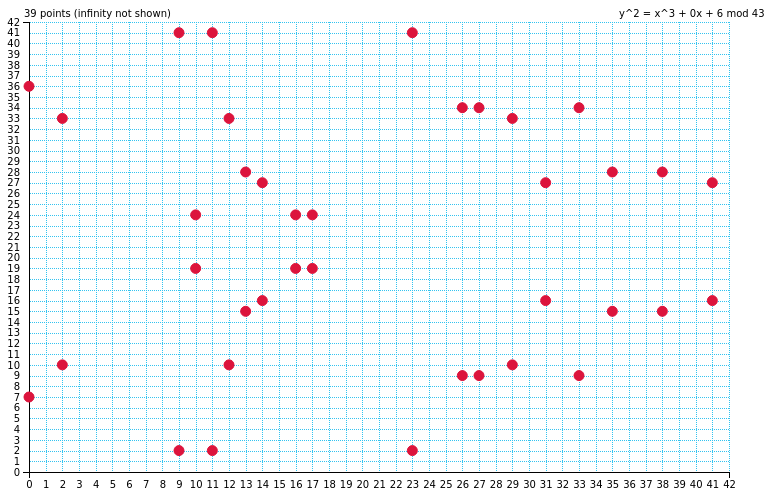
\includegraphics[scale=0.6]{figures/bls6-6.png}
As we can see our curve is somewhat nice, as it does not contain self inverse points that is points with $y=0$. It follows that the addition law can be optimized, since the branch for those cases can be eliminated. 

Note: Is there a way to printe the entire addition table from https://graui.de/code/elliptic2/ here? Would be nice to have but is a bit large.

Since the order of BLS6-6 is $39= 3\cdot 13$, we know that it has a "large" subgroup of order $13$ and small subgroup of order $3$. We can use XXX to find those groups. We have $BLS6-6(3)=\{\mathcal{O},(0,7),(0,36)\}$.

In addition we have the generator $g_{BLS6}:=(13,15)$ that generates
\begin{multline}
BLS6-6(13)=\\
\{(13,15) \rightarrow (33,34) \rightarrow  (38,15) \rightarrow  (35,28) \rightarrow (26,34) \rightarrow  (27,34) \rightarrow  \\ 
(27,9)  \rightarrow  (26,9) \rightarrow  (35,15) \rightarrow  (38,28) \rightarrow  (33,9) \rightarrow (13,28) \rightarrow  \mathcal{O}\}$$
\end{multline}

Computations "in the exponent": In cryptography and in particular in snarks a lot HAPPENS IN THE EXPONENT...

To use our example to explain what this means observe that from this representation, we can deduce a map from the scalar field $\F_{13}$ to $BLS6-6(13)$ with respect to our generator. WE have
$$
[\cdot]_{(13,15)}: \F_{13} \to BLS6-6(13)\;;\; x \mapsto [x](13,15)
$$

So for example we have $[1]_{(13,15)}= (13,15)$, $[7]_{(13,15)}= (27,9)$ and $[0]_{(13,15)}= \mathcal{O}$. In particular this map is a homomorphism of groups from the additive group $\F_{13}$ to $BLS6-6(13)$. This means in particular, the the additive neutral element from $\F_{13}$ is mapped to $\mathcal{O}$ and negatives are mapped to inverses. For example $[-2]_{(13,15)}= - [2]_{(13,15)}$, since
$[-2]_{(13,15)}= [11]_{(13,15)}= (33,9) = (33,-34) = -(33,34)=
- [2]_{(13,15)}$

The map also give a visualization of the ECDL problem in $BLS6-6(13)$, which is concerned with finding solutions $x\in \F_{13}$ for the equation 
$[x]_{(13,15)}= (x,y)$ for any $(x,y) \in BLS6-6(13)$. Of course ECDL is not hard in $BLS6-6(13)$, since we can deduce the solutions easily from XXX. For example the solution to $[x]_{(13,15)}= (35,15)$ is $x=9$, since $[9](13,15)=(35,15)$.

Since $[0]_{(13,15)}$ maps the group of cyclic integers modulo $13$ onto our group $BLS6-6(13)$, we can use this to write down the group law in the following way:
\begingroup
    \fontsize{5pt}{5pt}\selectfont
$$
\begin{array}{c|ccccccccccccc}
\cdot & \mathcal{O}  & (13,15) & (33,34) & (38,15) & (35,28) & (26,34) & (27,34) & (27,9) & (26,9) & (35,15) & (38,28) & (33,9) & (13,28)\\
\hline
\\
\mathcal{O} & \mathcal{O}  & (13,15) & (33,34) & (38,15) & (35,28) & (26,34) & (27,34) & (27,9) & (26,9) & (35,15) & (38,28) & (33,9) & (13,28)\\
\\
(13,15) & (13,15) & (33,34) & (38,15) & (35,28) & (26,34) & (27,34) & (27,9) & (26,9) & (35,15) & (38,28) & (33,9) & (13,28) & \mathcal{O}\\
\\
(33,34) & (33,34) & (38,15) & (35,28) & (26,34) & (27,34) & (27,9) & (26,9) & (35,15) & (38,28) & (33,9) & (13,28) & \mathcal{O} & (13,15)\\
\\
(38,15) & (38,15) & (35,28) & (26,34) & (27,34) & (27,9) & (26,9) & (35,15) & (38,28) & (33,9) & (13,28) & \mathcal{O} & (13,15) & (33,34)\\
\\
(35,28) & (35,28) & (26,34) & (27,34) & (27,9) & (26,9) & (35,15) & (38,28) & (33,9) & (13,28) & \mathcal{O} & (13,15) & (33,34) & (38,15)\\
\\
(26,34) & (26,34) & (27,34) & (27,9) & (26,9) & (35,15) & (38,28) & (33,9) & (13,28) & \mathcal{O} & (13,15) & (33,34) & (38,15) & (35,28)\\
\\
(27,34) & (27,34) & (27,9) & (26,9) & (35,15) & (38,28) & (33,9) & (13,28) & \mathcal{O} & (13,15) & (33,34) & (38,15) & (35,28) & (26,34)\\
\\
(27,9) & (27,9) & (26,9) & (35,15) & (38,28) & (33,9) & (13,28) & \mathcal{O} & (13,15) & (33,34) & (38,15) & (35,28) & (26,34) & (27,34)\\
\\
(26,9) & (26,9) & (35,15) & (38,28) & (33,9) & (13,28) & \mathcal{O} & (13,15) & (33,34) & (38,15) & (35,28) & (26,34) & (27,34) & (27,9)\\
\\
(35,15) & (35,15) & (38,28) & (33,9) & (13,28) & \mathcal{O} & (13,15) & (33,34) & (38,15) & (35,28) & (26,34) & (27,34) & (27,9) & (26,9)\\
\\
(38,28) & (38,28) & (33,9) & (13,28) & \mathcal{O} & (13,15) & (33,34) & (38,15) & (35,28) & (26,34) & (27,34) & (27,9) & (26,9) & (35,15)\\
\\
(33,9) & (33,9) & (13,28) & \mathcal{O} & (13,15) & (33,34) & (38,15) & (35,28) & (26,34) & (27,34) & (27,9) & (26,9) & (35,15) & (38,28)\\
\\
(13,28) & (13,28) & \mathcal{O} & (13,15) & (33,34) & (38,15) & (35,28) & (26,34) & (27,34) & (27,9) & (26,9) & (35,15) & (38,28) & (33,9)\\
\end{array}
$$
\endgroup


Cofactor clearing: 

Given an arbitrary point on the curve that is not in any of our two subgroups like $(2,33)$, we can project it on both subgroups $BLS6-6(3)$ and $BLS6-6(13)$ respectively, by \textit{multiplication with the cofactor}. Since $39 = 3 \cdot 13$, we have to multiply $(2,33)$ with $13$ to map it onto $BLS6-6(3)$ and we have to multiply $(2,33)$ with $3$ to map it onto $BLS6-6(13)$. Indeed we get $[13](2,33)= (0,36)$ which is an element of $BLS6-6(3)$ and $[3](2,33)= (35,15)$ which is an element of $BLS6-6(13)$

In what follows we want to compute type 2 pairings on our BLS6 curve. We therefore need to extract the subgroup $\mathbb{G}_1$ as well as $\mathbb{G}_2$ from the full $13$-torsion group. We already know from XXX that $\mathbb{G}_1$ is given by  
\begin{multline*}
\mathbb{G}_1=\{(13,15) \rightarrow (33,34) \rightarrow  (38,15) \rightarrow  (35,28) \rightarrow (26,34) \rightarrow  (27,34) \rightarrow  \\ 
(27,9)  \rightarrow  (26,9) \rightarrow  (35,15) \rightarrow  (38,28) \rightarrow  (33,9) \rightarrow (13,28) \rightarrow  \mathcal{O}\}$$
\end{multline*}

In type 2 pairings, the group $\mathbb{G}_2$ is defined by those elements $P$ of the full $13$-torsion group, that are mapped to $43\cdot P$ under the Frobenius endomorphism XXX. Since $BLS6/\F_{13^6}$ contains $6321251664$ elements, we can not simply loop through all elements, to find the full $13$-torsion group and extract all elements from $\mathbb{G}_2$. However we can derive the full $13$-torsion as the set of all $13$-division points and then extract $G_2$ from this
\begin{sagecommandline}
sage: F43 = GF(43)
sage: F43t.<t> = F43[]
sage: F43_6.<v> = GF(43^6, name='v', modulus=t^6+6) # t^6+6 irreducible
sage: BLS6 = EllipticCurve (F43_6,[0 ,6])
sage: INF = BLS6(0) # point at infinity
sage: for P in INF.division_points(13): # PI(P) == [q]P
....:     if P.order() == 13: # exclude point at infinity
....:         PiP = BLS6([a.frobenius() for a in P])
....:         qP = 43*P
....:         if PiP == qP:
....:             print(P.xy())
\end{sagecommandline}

Choose $g_2=(7v^2, 16v^3)$ as generator of $\mathbb{G}_2$, we get
\begin{multline*}
\mathbb{G}_2=\{
(7v^2, 16v^3) \to
(10v^2, 28v^3)\to
(42v^2, 16v^3)\to
(37v^2, 27v^3)\to\\
(16v^2, 28v^3)\to
(17v^2, 28v^3)\to
(17v^2, 15v^3)\to
(16v^2, 15v^3)\to\\
(37v^2, 16v^3)\to
(42v^2, 27v^3)\to
(10v^2, 15v^3)\to
(7v^2, 27v^3)\to
\mathcal{O}\}
\end{multline*}
e.g. $[3]g_2= (42v^2, 16v^3)$.

Having those groups we can do pairings. We choose the Weil pairing and invoke sagemath. For example the Weil pairing between our two generators is
$$
e(g_1,g_2)= 5v^5 + 16v^4 + 16v^3 + 15v^2 + 3v + 41
$$

\begin{sagecommandline}
sage: g1 = BLS6([13,15])
sage: g2 = BLS6([7*v^2, 16*v^3])
sage: g1.weil_pairing(g2,13)
\end{sagecommandline}

As we have seen, $\mathbb{G}_2$ needs quite a bit more storage space then $\mathbb{G}_1$, since elements in $\mathbb{G}_2$ are pairs of polynomials of degree $<6$ with coefficients in $\F_{43}$, while elements from $\mathbb{G}_1$ are just pairs of elements from $\F_{43}$. 

As we know from XXX it is possible to reduce the space needed to store $\mathbb{G}_2$ by using the concept of a twist. In our case $BLS6$ has embedding degree $6$ and the curve parameter $a$ in $y^2 = x^3 +ax + b$ is zero. We therefore know from XXX, that BLS6 has three different twist: A quadratic twist, a cubic twist and a sextic twist. We want to compute all of these twist:

The quadratic twisted BLS6-6 curve: Consider our BLS6-6 curve $BLS6-6/\F_{43^6}$. A quadratic twist is then another curve $BLS6-6_{2-twist}$ over $\F_{43^3}$ isomorphic to the original curve. We use XXX. The task is to find an $\omega\in \F_{43^6}$, such that $\omega^2 \in \F_{43^3}$. 
We choose $\omega = x^4 + 7x^3 + 9x^2 + 11x + 8$. Then we interpret $\delta = \omega^2 = 27x^2 + 17x + 35$ as an element from $\F_{43^3}$. So our twisted curve is
$y^2 = x^3+a\delta^2 x+b \delta^3 = x^3+6\cdot(27t^2+17t+35)$
so we get
$$
BLS6-6_{2-twist}/\F_{43^3}: y^2 = x^3+(10t^2+14t+15)
$$
\subsubsection{Baby JubJub}
% As we talk about R1CS already may write elliptic curves chapter after circuits/r1cs?
To give an understanding what the Baby-JubJub curve is, we want to parallel its development here to find a Baby-Jubjub like curve for pen and paper.

As with the original large Baby-JubJub curve we apply the method from
%https://www.hjp.at/doc/rfc/rfc7748.html#page_19 (Appendinx A)
to define a pen\& paper Baby-JubJub-like curve over the scalar field of the "large" BLS6 prime order subgroup, which is $\F_{13}$. 

Since $\Zmod{13}{4}=1$ we would go with A.1. As we will only find a few curves, we will tweak the algorithm and run
\begin{sagecommandline}
sage: F13 = GF(13) 
sage: for A in xrange(3, 13):
....:     if (A-2) % 4 != 0:
....:         continue
....:     try:
....:         E = EllipticCurve(F13, [0, A, 0, 1, 0]) # Montgomery form
....:         E
....:         E.order()
....:     except:               
....:         continue      
\end{sagecommandline}
So we get two curves in Montgomery form $y^2 = x^3 + 6*x^2 + x$ which has order $8$ and  $y^2 = x^3 + 10*x^2 + x$, which has order $16$. We could transform one of them into an Edwards curve, however   

So to find our Edwards curve, we will do exhaustive search rather 
\begin{sagecommandline}
sage: for d in F13:          
....:     j= ZZ(0)          
....:     for x in F13:
....:         for y in F13:                        
....:             if x^2+y^2 == 1+d*x^2*y^2:                           
....:                 j=j+1        
....:     print('d=',d)                
....:     print('order=',j)     
\end{sagecommandline}
and get $x^2+y^2= 1+7\cdot x^2y^2$ which has $20$ points. The associated Montgomery curve is then using XXX given by $8y^2 = x^3 + 6\cdot x^2 + x$.

So we define our Baby-JubJub Edwards curve to be
$$
EdBJJ/\F_{13}: x^2+y^2= 1+7\cdot x^2y^2
$$
with associated Montgomery form to be
$$
MBJJ/\F_{13}:8y^2 = x^3 + 6\cdot x^2 + x
$$
As $20=2\cdot 2\cdot 5$, we have a "large" prime order subgroup of order $5$ and a cofactor $4$. The group of rational points is
\begin{sagecommandline}
sage: for x in F13:                                   
....:     for y in F13:                                                                                
....:         if x^2+y^2 == F13(1)+F13(7)*x^2*y^2:                                                     
....:             print(x,y)
\end{sagecommandline}

$$
(0, 1),
(0, 12),
(1, 0),
(2, 4),
(2, 9),
(4, 2),
(4, 11),
(5, 6),
(5, 7),
(6, 5),
(6, 8),
(7, 5),
(7, 8),
(8, 6),
(8, 7),
(9, 2),
(9, 11),
(11, 4),
(11, 9),
(12, 0)
$$
with neutral element $(0,12)$

As expected we have a prime order subgroup of size $5$, which can be generated by $(11,9)$. We get $\{(11,9)\to (6,8)\to (7,8) \to (2,9) \to (0,1))\}$.

% rewrite into something nice
\begin{sagecommandline}
sage: def Edwards_add((x1,y1),(x2,y2),d):
....:     x3 = F13((F13(x1)*F13(y2)+F13(y1)*F13(x2))/((F13(1)+F13(d)*F13(x1)*F13
....: (x2)*F13(y1)*F13(y2))))
....:     y3 = F13((F13(y1)*F13(y2)-F13(x1)*F13(x2))/((F13(1)-F13(d)*F13(x1)*F13
....: (x2)*F13(y1)*F13(y2))))
....:     return (x3,y3)
\end{sagecommandline}

\paragraph{Hashing to the pairing groups}
We give various constructions to hash into $\mathbb{G}_1$ and $\mathbb{G}_2$. 

We start with hashing to the scalar field... TO APPEAR

Non of these techniques work for hashing into $\mathbb{G}_2$. We therefore implement Pederson's Hash for BLS6. 

We start with $\mathbb{G}_1$. Our goal is to define an $12$-bit bounded hash function
$$
H_{1}: \{0,1\}^{12} \to \mathbb{G}_1 
$$
Since $12= 3\cdot 4$ we "randomly" select $4$ uniformly distributed generators $\{(38, 15), (35,28), (27, 34), (38, 28)\}$ from $\mathbb{G}_1$ and use the pseudo-random function from XXX. 
For every genrator we therefore have to choose a set of $4$ randomly generated invertible elements from $\F_{13}$. We choose
$$
\begin{array}{lcl}
(38,15) &:& \{2,7,5,9\}\\
(35,28) &:& \{11,4,7,7\}\\
(27,34) &:& \{5,3,7,12\}\\
(38,28) &:& \{6,5,1,8\}
\end{array}
$$
So our hash function is computed like this:
\begin{multline*}
H_1(x_{11},x_1,\ldots, x_{0})=
[2\cdot 7^{x_{11}}\cdot 5^{x_{10}}\cdot 9^{x_9}](38,15)+
[11\cdot 4^{x_8}\cdot 7^{x_7}\cdot 7^{x_6}](35,28)+\\
[5\cdot 3^{x_5}\cdot 7^{x_4}\cdot 12^{x_3}](27,34) +
[6\cdot 5^{x_2}\cdot 1^{x_{1}}\cdot 8^{x_{0}}](38,28)
\end{multline*}
Note that $a^x=1$ whe $x=0$ and hence those terms can be omitted in the computation. 
In particular the hash of the $12$-bit zero string is given by 
\begin{multline*}WRONG-ORDERING-REDO
H_1(0)= [2](38,15)+[11](35,28)+[5](27,34)+[6](38,28)= \\
(27,34)+(26,34)+(35,28)+(26,9)= (33,9) + (13,28) = (38,28)
\end{multline*}
The hash of $011010101100$ is given by 
\begin{multline*}
H_1(011010101100)=WRONG-ORDERING-REDO\\
[2\cdot 7^{0}\cdot 5^{1}\cdot 9^{1}](38,15)+
[11\cdot 4^{0}\cdot 7^{1}\cdot 7^{0}](35,28)+
[5\cdot 3^{1}\cdot 7^{0}\cdot 12^{1}](27,34) +
[6\cdot 5^{1}\cdot 1^{0}\cdot 8^{0}](38,28)=\\
[2\cdot 5\cdot 9](38,15)+
[11\cdot 7](35,28)+
[5\cdot 3\cdot 12](27,34) +
[6\cdot 5](38,28)=\\
[12](38,15)+
[12](35,28)+
[11](27,34) +
[4](38,28)=\\ 
TO_APPEAR
\end{multline*}
We can use the same technique to define a $12$-bit bounded hash function in $\mathbb{G}_2$:  
$$
H_{2}: \{0,1\}^{12} \to \mathbb{G}_2 
$$
Again we "randomly" select $4$ uniformly distributed generators $\{(7v^2 , 16v^3 ), (42v^2 , 16v^3 ), (17v^2 , 15v^3 ), (10v^2 , 15v^3 )\}$ from $\mathbb{G}_2$ and use the pseudo-random function from XXX. For every genrator we therefore have to choose a set of $4$ randomly generated invertible elements from $\F_{13}$. We choose
$$
\begin{array}{lcl}
(7v^2 , 16v^3 ) &:& \{8,4,5,7\}\\
(42v^2 , 16v^3 ) &:& \{12,1,3,8\}\\
(17v^2 , 15v^3 ) &:& \{2,3,9,11\}\\
(10v^2 , 15v^3 ) &:& \{3,6,9,10\}
\end{array}
$$
So our hash function is computed like this:
\begin{multline*}
H_1(x_{11},x_{10},\ldots, x_{0})=
[8\cdot 4^{x_{11}}\cdot 5^{x_{10}}\cdot 7^{x_9}](7v^2 , 16v^3)+
[12\cdot 1^{x_8}\cdot 3^{x_7}\cdot 8^{x_6}](42v^2 , 16v^3 )+\\
[2\cdot 3^{x_5}\cdot 9^{x_4}\cdot 11^{x_3}](17v^2 , 15v^3 ) +
[3\cdot 6^{x_2}\cdot 9^{x_{1}}\cdot 10^{x_{0}}](10v^2 , 15v^3 )
\end{multline*}
We extend this to a hash function that maps unbounded bitstring to $\mathbb{G}_2$ by precomposing with an actual haah function like $MD5$ and feet the first 12 bits of its outcome into our previously defined hash function. 
$$
TinyMD5_{\mathbb{G}_2}: \{0,1\}^* \to \mathbb{G}_2
$$
with $TinyMD5_{\mathbb{G}_2}(s)= H_2(MD5(s)_0,\ldots MD5(s)_{11})$. For example, since 
$MD5("")= 0xd41d8cd98f00b204e9800998ecf8427e$ and the binary representation of the hexadecimal number $0x27e$ is $001001111110$ we compute $TinyMD5_{\mathbb{G}_2}$ of the empty string as
$TinyMD5_{\mathbb{G}_2}("")= H_2(MD5(s)_{11},\ldots MD5(s)_{0}) = H2(001001111110)=$

\subsubsection{Baby-JubJub-2}
To give an understanding what the Baby-JubJub curve is, we want to parallel its development here to find a Baby-Jubjub like curve for pen and paper.

The original Baby-JubJub is a twisted Edwards curve over $\F_{?}$ with $a=-1$ and $d=?.$

As with the original large Baby-JubJub curve we apply the method from
%https://www.hjp.at/doc/rfc/rfc7748.html#page_19 (Appendinx A)
to define a pen\& paper Baby-JubJub-like curve over the scalar field of the "large" BLS6 prime order subgroup, which is $\F_{13}$. 

Since $\Zmod{13}{4}=1$ we would go with A.1. As we will only find a few curves, we will tweak the algorithm and run
\begin{sagecommandline}
sage: F13 = GF(13) 
sage: for A in xrange(3, 13):
....:     if (A-2) % 4 != 0:
....:         continue
....:     try:
....:         E = EllipticCurve(F13, [0, A, 0, 1, 0]) # Montgomery form
....:         E
....:         E.order()
....:     except:               
....:         continue      
\end{sagecommandline}
So we get two curves in Montgomery form $y^2 = x^3 + 6*x^2 + x$ which has order $8$ and  $y^2 = x^3 + 10*x^2 + x$, which has order $16$. We could transform one of them into an Edwards curve, however   

So to find our Edwards curve, we will do exhaustive search rather 
\begin{sagecommandline}
sage: j = ZZ(0)
sage: for a in F13:
....:     for d in F13:
....:         j = 0
....:         for x in F13:
....:             for y in F13:
....:                 if a*x^2 + y^2 == 1+d*x^2*y^2:
....:                     j=j+1
....:         print('curve: a=',a,'d=',d,'order:',j)     
\end{sagecommandline}
We want to choose a curve that has a large prime order subgroup and a small cofactor. So we go
with $2x^2+y^2= 1+3\cdot x^2y^2$ which has order $14$. 


The associated Montgomery curve is then using XXX given by $9y^2 = x^3 +2x^2 + x$.

So we define our Baby-JubJub Edwards curve to be
$$
EdBJJ/\F_{13}: 2x^2+y^2= 1+3\cdot x^2y^2
$$
with associated Montgomery form to be
$$
MBJJ/\F_{13}:9y^2 = x^3 + 2x^2 + x
$$
As $14=2\cdot 7$, we have a "large" prime order subgroup of order $7$ and a cofactor $2$. The group of rational points is
\begin{sagecommandline}
sage: for x in F13:                                   
....:     for y in F13:                                                                                
....:         if F13(2)*x^2+y^2 == F13(1)+F13(11)*x^2*y^2:                                                     
....:             print(x,y)
\end{sagecommandline}

$$
(0, 1),
(0, 12),
(2, 4),
(2, 9),
(4, 5),
(4, 8),
(5, 2),
(5, 11),
(8, 2),
(8, 11),
(9, 5),
(9, 8),
(11, 4),
(11, 9)
$$
with neutral element $(0,1)$

As expected we have a prime order subgroup of size $5$, which can be generated by $(11,9)$. We get $\{(11,9)\to (6,8)\to (7,8) \to (2,9) \to (0,1))\}$.

% rewrite into something nice
\begin{sagecommandline}
sage: def Edwards_add((x1,y1),(x2,y2),a,d):
....:     x3 = F13((F13(x1)*F13(y2)+F13(y1)*F13(x2))/((F13(1)+F13(d)*F13(x1)*F13(x2)*F13(y1)*F13(y2))))
....:     y3 = F13((F13(y1)*F13(y2)-F13(a)*F13(x1)*F13(x2))/((F13(1)-F13(d)*F13(x1)*F13(x2)*F13(y1)*F13(y2))))
....:     return (x3,y3)
\end{sagecommandline}




\subsection{MNT4 MNT6 Cycles}
% https://eprint.iacr.org/2006/372.pdf theorem 5.2
\begin{theorem}
Let $q$ be a prime and $E/\F_q$ be an ordinary elliptic curve such that $r= |E(Fq)|$ is a prime greater than $3$.  
\begin{itemize}
\item $E$ has embedding  degree $k= 4$ if and only if there  exists $x\in \mathbb{Z}$ such  that $t=-x$ or $t=x+1$, and $q=x^2+x+1$.\item $E$ has  embedding  degree $k= 6$ if and only if there  exists $x\in \Z$ such that $t= 1\pm 2x$ and $q=4x^2+1$.
\item There is an elliptic curve $E/\F_q$ with embedding degree $6$, discriminant $D$, and $|E(Fq)| = r$ if and only if there is an elliptic curve $E'/\F_r$ with embedding degree $4$, discriminant $D$, and $|E'(\F_r)| =q$.
\end{itemize}
\end{theorem}

We can use this theorem to find an MNT6-MNT4 cycle over very small prime fields with characteristics $>3$: 
\paragraph{MNT4}
For our MNT4 curve, we can choose $x=2$. Then $q=7$ and if we choose $t= x+1 $ then $r = q + 1 - t = 7 + 1 -3 = 5$. Therefore our MNT4 curve is a curve $y^2=x^3+ax+b$ defined over $\F_7$ that consists of $5$ points. 

To construct the actual curve we could use the complex multiplication method again, but since the parameters $a$ and $b$ are from $\F_7$ there are only $48$ possibilities so we simply loop through all possible $a$'s and $b$'s and count the curve points until we find a curve that has $5$ rational points. We get
$$
y^2 = x^3 + 4x + 1
$$
defined over $\F_7$, with scalar field $\F_5$. Since $7= 2^2+2+1$, we know from theorem XXX, that this curve has embedding degree $4$ and hence qualifies as a pen\&{}paper pairing friendly elliptic curve. Since the curve's order is a prime and therefore has no non trivial factors, it has no non trivial subgroups. The curve has the following set of elements
$$MNT4=\{(0,1)\to (0,6)\to (4,2)\to (4,5) \to \mathcal{O}\}$$ 
\begin{sagecommandline}
sage: F7 = GF(7)
sage: MNT4 = EllipticCurve (F7,[4 ,1])
sage: [P.xy() for P in MNT4.points() if P.order() > 1]
\end{sagecommandline}
The multiplication table is
\begingroup
    \fontsize{10pt}{10pt}\selectfont
$$
\begin{array}{c|ccccc}
\cdot & \mathcal{O} & (0,1) & (4,5) & (4,2) & (0,6)\\
\hline
\\
\mathcal{O} & \mathcal{O} & (0,1) & (4,5) & (4,2) & (0,6)\\
\\
(0,1) & (0,1) & (4,5) & (4,2) & (0,6) & \mathcal{O}\\
\\
(4,5) & (4,5) & (4,2) & (0,6) & \mathcal{O} & (0,1)\\
\\
(4,2) & (4,2) & (0,6) & \mathcal{O} & (0,1) & (4,5)\\
\\
(0,6) & (0,6) & \mathcal{O} & (0,1) & (4,5) & (4,2)\\
\end{array}
$$
\endgroup
In what follows we choose our generator to be $g_{MNT4}=(0,1)$.

In what follows we want to compute type 2 pairings on our MNT4 curve. We therefore need to extract the subgroup $\mathbb{G}_1$ as well as $\mathbb{G}_2$ from the full $5$-torsion group. Since the order of MNT4 is a prime number, we already know from XXX that $\mathbb{G}_1$ is given by  
$$\mathbb{G}_1=\{(0,1)\to (0,6)\to (4,2)\to (4,5) \to \mathcal{O}\}$$ 

In type 2 pairings, the group $\mathbb{G}_2$ is defined by those elements $P$ of the full $5$-torsion group, that are mapped to $7\cdot P$ under the Frobenius endomorphism XXX. Since $MNT4/\F_{7^4}$ only contains $2475$ elements, we can  loop through all elements, to find the full $5$-torsion group and extract all elements from $\mathbb{G}_2$:
\begin{sagecommandline}
sage: F7t.<t> = F7[]
sage: F7_4.<u> = GF(7^4, name='u', modulus=t^4+t+1) # embedding degree is 4
sage: MNT4 = EllipticCurve (F7_4,[4 ,1])
sage: INF = MNT4(0) # point at infinity
sage: for P in INF.division_points(5): # PI(P) == [q]P
....:     if P.order() == 5: # exclude point at infinity
....:         PiP = MNT4([a.frobenius() for a in P])
....:         qP = 7*P
....:         if PiP == qP:
....:             print(P.xy())
\end{sagecommandline}

Choose $g_2=(2u^3 + 5u^2 + 4u + 2, 2u^3 + 3u + 5)$ as generator of $\mathbb{G}_2$, we get
\begin{multline*}
\mathbb{G}_2=\{ 
(2u^3 + 5u^2 + 4u + 2, 2u^3 + 3u + 5) \to
(5u^3 + 2u^2 + 3u + 6, 2u^2 + 3u) \to \\
(5u^3 + 2u^2 + 3u + 6, 5u^2 + 4u) \to
(2u^3 + 5u^2 + 4u + 2, 5u^3 + 4u + 2)\to
\mathcal{O}\}
\end{multline*}
e.g. $[3]g_2= (5u^3 + 2u^2 + 3u + 6, 5u^2 + 4u)$.

Having those groups we can do pairings. We choose the Weil pairing and invoke sagemath. For example the Weil pairing between our two generators is
$$
e(g_1,g_2)= 5u^3 + 2u^2 + 6u
$$
\begin{sagecommandline}
sage: g1 = MNT4([0,1])
sage: g2 = MNT4(2*u^3 + 5*u^2 + 4*u + 2, 2*u^3 + 3*u + 5)
sage: g1.weil_pairing(g2,5)
\end{sagecommandline}
The full pairing table can the be written as
\begingroup
    \fontsize{10pt}{10pt}\selectfont
    
% generate the table entries as:
% sage: for i in range(5):
% ....:     for j in range(5):
% ....:         p = (i*g1).weil_pairing((j*g2),5)
% ....:         print('e([',i,']g1,[',j,']g2=',p)         
    
    
$$
\begin{array}{c|lllll}
e(\cdot,\cdot)    & \mathcal{O} & g_1            & [2]g_1         & [3]g_1         & [4]g_1\\
\hline
\\
      \mathcal{O} & 1           & 1              & 1              & 1              & 1\\
\\
              g_2 & 1           & 5u^3+2u^2+6u   & 6u^3+5u^2+6    & 2u^3+u^2+2u+3  & u^3+6u^2+6u+4\\
\\
\left[2\right]g_2 & 1           & 6u^3+5u^2+6    & u^3+6u^2+6u+4  & 5u^3+2u^2+6u   & 2u^3+u^2+2u+3\\
\\
\left[3\right]g_2 & 1           & 2u^3+u^2+2u+3  & 5u^3+2u^2+6u   & u^3+6u^2+6u+4  & 6u^3+5u^2+6\\
\\
\left[4\right]g_2 & 1           & u^3+6u^2+6u+4  & 2u^3+u^2+2u+3  & 6u^3+5u^2+6    & 5u^3+2u^2+6u\\
\end{array}
$$
\endgroup

\paragraph{MNT6}
For our MNT6 curve, we can choose $x=1$. Then $q=5$ and if we choose $t= 1 + 2x $ then $r= q + 1 - t = 5 + 1 + 1 = 7$. Therefore our MNT6 curve is a curve $y^2=x^3+ax+b$ defined over $\F_5$ that consists of $7$ points. 

To construct the actual curve we could use the complex multiplication method again, but since the parameters $a$ and $b$ are from $\F_5$ there are only $24$ possibilities, we simply loop through all possible $a$'s and $b$'s and count the curve points until we find a curve that has $7$ rational points. We get
$$
y^2 = x^3 + 2x + 1
$$
defined over $\F_5$. Since $5= 4\cdot 1 + 1$, we know from theorem XXX, that this curve has embedding degree $6$ and hence qualifies as a pen\&{}paper pairing friendly elliptic curve. 

The curve has the following set of elements
$$MNT6=\{(1,2)\to (3,3)\to (0,1)\to (0,4)\to (3,2)\to (1,3)\to \mathcal{O}\}$$
The multiplication table is
\begingroup
    \fontsize{10pt}{10pt}\selectfont
$$
\begin{array}{c|ccccccc}
\cdot & \mathcal{O} & (1,2) & (3,3) & (0,1) & (0,4) & (3,2) & (1,3)\\
\hline
\\
\mathcal{O} & \mathcal{O} & (1,2) & (3,3) & (0,1) & (0,4) & (3,2) & (1,3)\\
\\
(1,2) & (1,2) & (3,3) & (0,1) & (0,4) & (3,2) & (1,3) & \mathcal{O}\\
\\
(3,3) & (3,3) & (0,1) & (0,4) & (3,2) & (1,3) & \mathcal{O} & (1,2)\\
\\
(0,1) & (0,1) & (0,4) & (3,2) & (1,3) & \mathcal{O} & (1,2) & (3,3)\\
\\
(0,4) & (0,4) & (3,2) & (1,3) & \mathcal{O} & (1,2) & (3,3) & (0,1)\\
\\
(3,2) & (3,2) & (1,3) & \mathcal{O} & (1,2) & (3,3) & (0,1) & (0,4)\\
\\
(1,3) & (1,3) & \mathcal{O} & (1,2) & (3,3) & (0,1) & (0,4) & (3,2)\\
\end{array}
$$
\endgroup

In what follows we choose our generator to be $g_{MNT6}=(1,2)$.

In what follows we want to compute type 2 pairings on our MNT6 curve. We therefore need to extract the subgroup $\mathbb{G}_1$ as well as $\mathbb{G}_2$ from the full $7$-torsion group. Since the order of MNT6 is a prime number, we already know from XXX that $\mathbb{G}_1$ is given by
$$\mathbb{G}_1=\{(1,2)\to (3,3)\to (0,1)\to (0,4)\to (3,2)\to (1,3)\to \mathcal{O}\}$$
In type 2 pairings, the group $\mathbb{G}_2$ is defined by those elements $P$ of the full $7$-torsion group, that are mapped to $5\cdot P$ under the Frobenius endomorphism XXX. Since $MNT6/\F_{5^6}$ contains $15680$ elements, we can still loop through all elements, to find the full $7$-torsion group and extract all elements from $\mathbb{G}_2$

\begin{sagecommandline}
sage: G.<x> = GF(5^6) # embedding degree is 6
sage: MNT6 = EllipticCurve (G,[2 ,1])
sage: INF = MNT6(0) # point at infinity
sage: for P in INF.division_points(7): # PI(P) == [q]P
....:     if P.order() == 7: # exclude point at infinity
....:         PiP = MNT6([a.frobenius() for a in P])
....:         qP = 5*P
....:         if PiP == qP:
....:             print(P.xy())
\end{sagecommandline}

\begin{multline*}
\mathbb{G}_2=\{ 
(x^3+2x^2+4x,x^5+2x^4+4x^3+3x^2+3)\to
(x^5+4x^4+2x^3+3x^2+x+2,3x^4+2x^3+x)\to\\
(4x^5+x^4+2x^3,3x^5+x^4+x^3+4x+4)\to
(4x^5+x^4+2x^3,2x^5+4x^4+4x^3+x+1) \to\\
(x^5+4x^4+2x^3+3x^2+x+2,2x^4+3x^3+4x)\to
(x^3+2x^2+4x,4x^5+3x^4+x^3+2x^2+2)\to
\mathcal{O}\}
\end{multline*}
We choose the generator $g_2 = (x^3+2x^2+4x,x^5+2x^4+4x^3+3x^2+3)$

\begin{remark}
Note however that our MNT6 curve discriminant $D=-16(4a^3 + 27 b^2)= -16(4\cdot 2^3 + 27\cdot 1^2)=-944$, while our MNT4 curve has discriminsnt XXX. Hence our example curves are not those guranteed by theorem XXX. Those curve are both given by $y^2= x^3 + 2x +1$ over $\F_5$ and $\F_7$, respectively. However as both curves have the same defining equation, we rather choose examples that are visually distinguishable by their defining equations.
\end{remark}

\subsection{Edwards curve cycles}
